\newcommand{\labtitle}{ECE/CS 5710/6710 - Lab 5}
\newcommand{\labsubtitle}{Floorplanning and Place $\&$ Route of a MIPS Processor}
\vlsiheader

\begin{center}
	\LARGE\textbf{\labsubtitle} \\
	\large\textbf{Pre-lab Assignment:} Check for the date on Canvas. \\
	\large\textbf{Lab Report:} Check for the date on Canvas.
\end{center}
\section{Objective}
This lab presents the main steps for performing the Place $\&$ Route (P$\&$R) step of the 8-bit MIPS microprocessor you synthesized in the previous lab, using the TSMC 180 \emph{nm} design kit. This lab details the typical steps of the back-end flow in VLSI design: floorplan, placement, clock tree synthesis and routing. The tool you will use is Cadence Innovus\textsuperscript{\tiny\textregistered}, which is widely used in industry and academia. Innovus being a very complete and complicated tool, you will only use its basic functions in this lab, but remember that many other options and optimizations are available for each step.
\begin{remark}
Note that this lab has been written with the verilog gate-level netlist obtained after the synthesis step with a very relaxed timing constraint. As such, some values such as the timing reports may differ from what you will get. Also, keep in mind that while your synthesized design was meeting your timing constraint, it might not meet it anymore after the P$\&$R flow. In that case, you need to re-synthesized it with a more relaxed timing constraint and redo the P$\&$R flow.
\end{remark}

%Before starting this lab, it is suggested that you run the \textit{synthesis.tcl} script from the previous lab with a large timing constraint to begin with (such as 15ns for the \textit{clk} period). You will then refine and optimize your design in the last part of this lab.	

\section{Pre-lab Assignment}

\begin{prelab}
	Answer the following question and submit a \textbf{.pdf} file through Canvas:
	\begin{enumerate}
	\item What is the difference between a semi-custom and a full-custom design?
	\item Describe briefly the main steps of the back-end flow.
	\item What are clock jitter and clock skew and how can they be minimized?
	\item What does the core density of your chip depend on?
	\item What is IR drop? How can it be mitigated?
	\end{enumerate}
	\vspace{-5mm}
\end{prelab}


\section{Directory Organization}
For the Place $\&$ Route flow, you will have to work in your \textit{innovus} folder. This folder contains different subdirectories as follows:
 \begin{itemize}
\item \textit{DBS}: design database, where you will save your design after the different step of the P$\&$R.
\item \textit{RPT}: report files (area, number of gates, hierarchy etc.) created by the tool.
\item \textit{CONF}: Design import configuration files.
\item \textit{SCRIPTS}: Contains some script(s) used in this lab.
\item \textit{GDS}: Used to export your final design as a GDSII file.
\item \textit{SDF}: Timing files created by the tool for functional verification.
\end{itemize}

\section{Lab Assignment}
\subsection{Starting Cadence Innovus\textsuperscript{\tiny\textregistered}}
Launch the Cadence Innovus\textsuperscript{\tiny\textregistered} GUI by going in your \textit{innovus
} folder and doing:
	\begin{codeline}
	innovus
\end{codeline}



You will obtain a window as shown in Fig \ref{fig_main_window}. The console terminal is used for entering Innovus\textsuperscript{\tiny\textregistered} commands, to source Tcl scripts or to run Linux commands. Pay attention to it since it contains crucial information when something went wrong in your flow (everything displayed in the current terminal is also stored in the \textit{innovus.log} file in the \textit{innovus} directory. \textbf{In case of errors, it is very helpful to open this \textit{.log} in a text editor in order to check what went wrong}). When you will perform actions on the GUI, the equivalent commands will be recorded and stored in the \textit{innovus.cmd} file in the \textit{innovus} directory. The equivalent commands will also be given in this tutorial.
\begin{figure}[!h]
	\centering
	\includegraphics[scale=0.33]{figures/lab5_backend/innovus_main_windows.pdf}
	\caption{Cadence Innovus window organization.}
	\label{fig_main_window}
\end{figure}

The main window includes three different design views: the Floorplan view, the Amoeba view, and the Physical view. You can switch the view whenever you want by clicking on the icon view, as shown in Fig. \ref{fig_switch_view}.
\begin{itemize}
	\parbox[t]{\dimexpr\textwidth-\leftmargin}{%
	\begin{wrapfigure}[9]{r}{0.4\textwidth}
		\vspace{0mm}
		\centering
		\vspace{-\baselineskip}
	
\includegraphics[scale=1]{figures/lab5_backend/switch_view}
\caption{Switch the design view}
\label{fig_switch_view}
	\end{wrapfigure}
	\item \textit{The Floorplan view} displays the hierarchical module and block guides, floorplan objects, the connection lines and power/ground nets.
	\item \textit{The Amoeba view} displays the outline of the modules and submodules after placement, showing the physical locality of the module.
}
	\item \textit{The Physical view} displays the detailed placements of the module blocks, standard cells, nets, and interconnects.
\end{itemize}

As in Virtuoso\textsuperscript{\tiny\textregistered}, there are many useful shortcuts you can use. The most important ones are presented in Table \ref{shortcuts}. 
\begin{table}[h!]
	\caption{Main Innovus\textsuperscript{\tiny\textregistered} shortcuts.}
	\label{shortcuts}
\centering
	\begin{tabular}{ |c| c| }
				\hline
		\textbf{Shortcut} & \textbf{Action}  \\ 
		\hline
		b & display the list of binding keys  \\  
				\hline
		d & (de)select or delete objects    \\
				\hline
				f & zoom the display to fit the core area\\
\hline
g& ascend in hierarchy\\
\hline
shift+g& descend in hierarchy\\
\hline
k &create a ruler\\
\hline
maj+k & remove last ruler displayed\\
\hline
q display & the object attribute editor form for the selected object. \\
&click the left-button mouse to select an object\\
&shift-click to select or deselect an object\\
\hline
u & undo last command\\
\hline
shift+u & redo last command\\
\hline
z & 2$\times$ zoom-in\\
\hline
shift+z & 2$\times$zoom-out\\
\hline
shift+ctrl+r& refresh the display\\
\hline
	\end{tabular}
\end{table}



\subsection{Defining the Design Import Configuration}
Before starting the P$\&$R steps, you must import all the different files:
\begin{itemize}
	\item \textit{Technology information (\textit{.lef} files)}: those files include the technology process design rules for placement and routing (name, spacing, width of routing layers, vias definition, core and pad site definitions, placement orientation \textit{etc.}) and the physical informations about the standard cells (width and height, used metals etc.). Those files are supplied by the library cell provider.
	\item \textit{Timing libraries}: those files contain the timing information for all the standard cells (path delays, setup and hold times \textit{etc.}). Those are the same files you used in Synopsys DC\textsuperscript{\tiny\textregistered} but here in the Liberty text (\textit{.lib}) format. Those files are supplied by the library cell provider.
	\item \textit{Capacitance tables}: Those files contains the necessary information for accurate capacitance extraction for the routing preparation and optimization steps. The tables are generally supplied as text files without standard file extension (e.g., .CapTbl) by the foundry, or can be generated with the process design kit.
	\item \textit{Gate-level netlist}: this is the design netlist (\textit{.v}) which will be placed and routed. This file has been generated during the synthesis (in the previous lab).
	\item \textit{Timing constraints}: this file (\textit{.sdc}) relates to the constraints you used during the synthesis and has been generated by Synopsys DC\textsuperscript{\tiny\textregistered}.
\end{itemize}


	\parbox[t]{\dimexpr\textwidth-\leftmargin}{%
		\begin{wrapfigure}[24]{r}{0.5\textwidth}
			\vspace{0mm}
			\centering
			\vspace{-\baselineskip}
		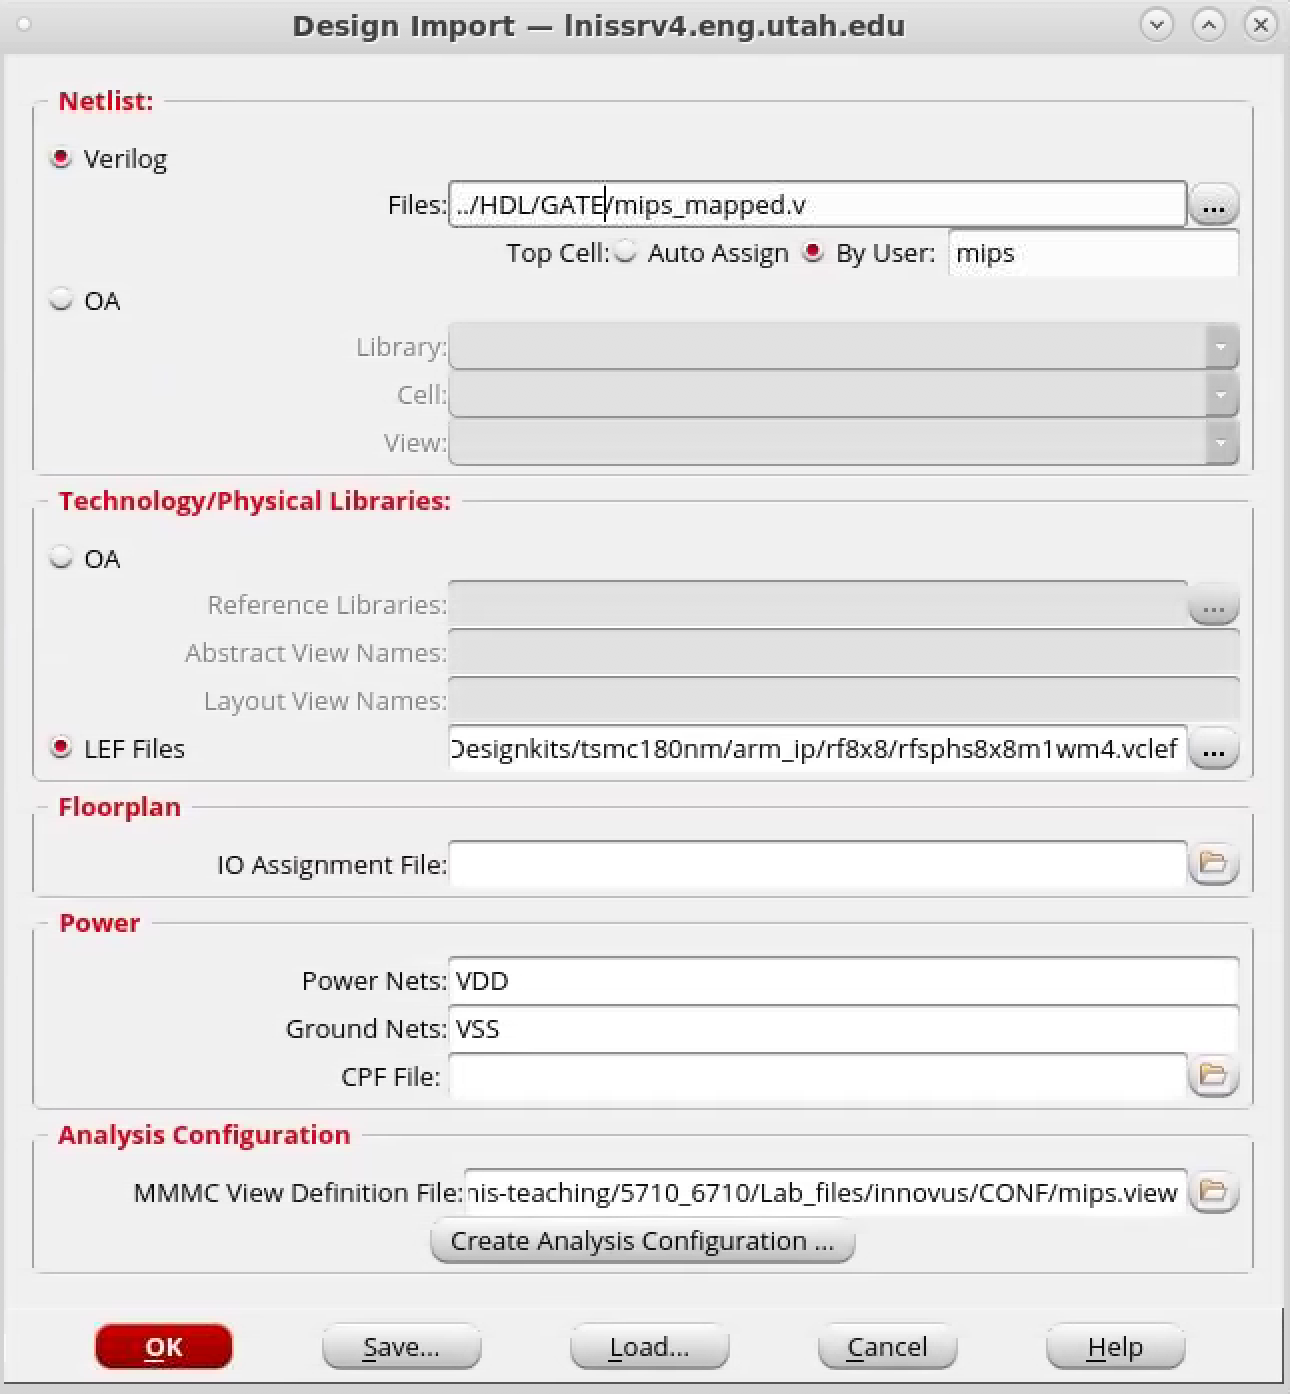
\includegraphics[scale=0.35]{figures/lab5_backend/mmmc}
\caption{Design import window.}
\label{fig_mmmcview}
		\end{wrapfigure}
The first task is to create a design configuration file which will define all the previous file in order to properly load the design for the back-end steps. Once such a configuration file exists, it can be simply loaded to import the design directly. To do so:

\begin{enumerate}
	\item \textit {File -> Import Design...} 
	\item Click on the \textit{Load...} button, as shown in Fig \ref{fig_mmmcview} and load the \textit{CONF/mips.globals} file. After this step, some settings should be applied to the design import window.
	The loaded file includes some configuration file for the TSMC 180 \textit{nm} process. In particular, it contains the information and paths to the \textit{.lib} and \textit{.lef} files from the TSMC library required by the P$\&$R tool. It also contains the path to your synopsys \textit{.sdc} file so you will not need to add it yourself in the configuration step.
\end{enumerate}
	}
			\vspace{5mm}


 \begin{enumerate}
	\parbox[t]{\dimexpr\textwidth-\leftmargin}{%
	\begin{wrapfigure}[24]{r}{0.5\textwidth}
		\vspace{0mm}
		\centering
		\vspace{-\baselineskip}
		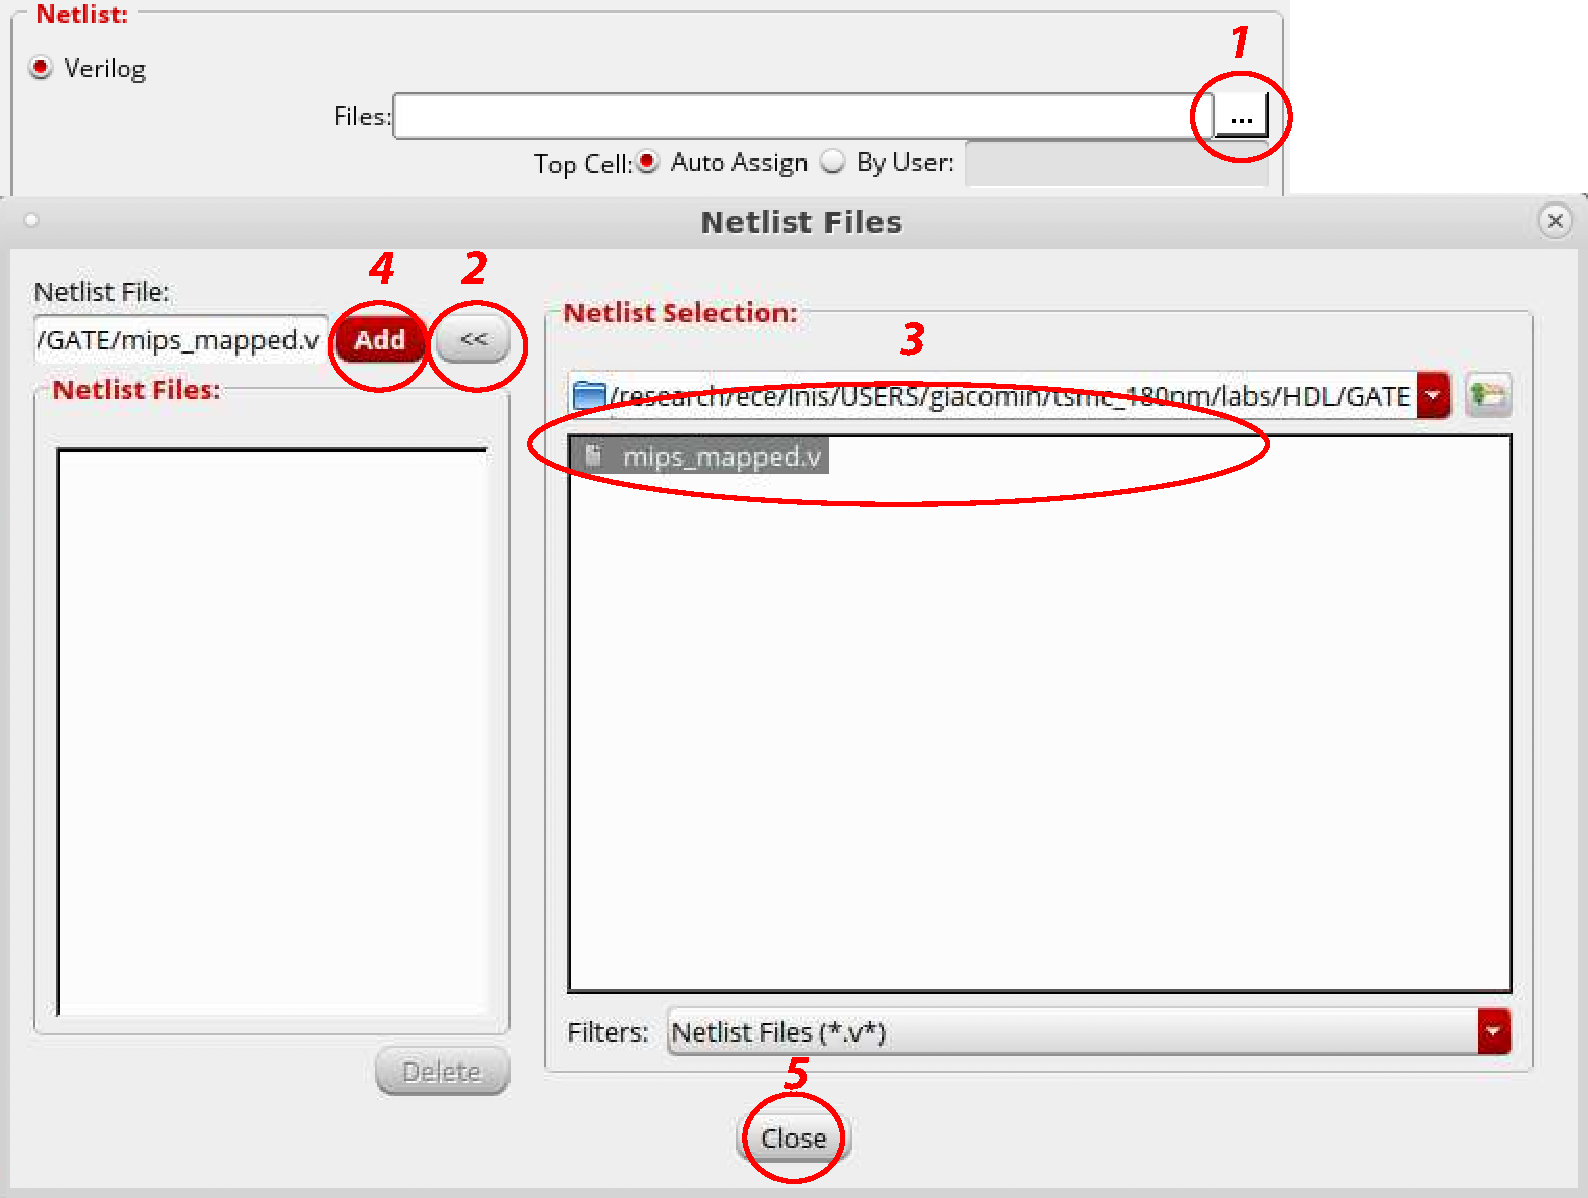
\includegraphics[scale=0.31]{figures/lab5_backend/addverilog.pdf}
\caption{Adding the gate-level verilog file.}
\label{fig_addverilog}
	\end{wrapfigure}
The design import phase still needs to be completed with the design data which is to be placed and routed. More particularly, you need to add the gate-level Verilog file netlist you synthesized in the previous lab:
	\item From the design import window, next to the \textit{Verilog} field, click on the \textbf{...} button as illustrated in Fig. \ref{fig_addverilog}.
\item Click on the \textbf{$>>$} button to get the \textit{Netlist Selection} pane. Select the Verilog gate-level netlist in \textit{HDL/GATE/mips$\_$mapped.v}.

\item Click on \textit{Add} then \textit{Close}. 
}
\clearpage
	\item Next, fill the \textit{Power Nets} and \textit{Ground Nets} fields by $VDD$ and $VSS$ respectively, as in Fig. \ref{fig_mmmcview}.
	\item From the design import window, click on \textit{Save} to save your configuration as \textit{mips$\_$final.globals} in the \textit{CONF} directory. In case you need to modify some configuration later on, it will save all the settings you defined.
\item Finally, click on the \textit{OK} button from the design import window the perform the design importation.
		\vspace{-6mm}
\begin{remark}
	It is important to check that everything went smoothly after the importing step. Check the terminal to see if there was any error (a summary should be displayed at the very last lines of the terminal). If there is one, you need to check what went wrong by scrolling up into the terminal (you might have specified a wrong verilog file path for instance).
\end{remark}
	\vspace{-4mm}
\end{enumerate}

\subsection{Importing the Design}

This step needs only to be done when you will launch Innovus\textsuperscript{\tiny\textregistered} again, to reload your design in its initial configuration. To import directly the design, without doing the previous step:
 \begin{enumerate}
	\item Go to \textit{File -> Import Design...}
	\item Click on the \textit{Load..} button and select the \textit{mips$\_$final.globals} in the \textit{CONF} directory.
	\item Click on \textit{OK}.
\end{enumerate}


Equivalent Innovus command:
	\begin{codeline}
source CONF/mips$\_$final.globals \\
init$\_$design
\end{codeline}


\subsection{Saving and Restoring the Design}\label{save}
The back-end flow contains several steps. Therefore, it is important to save your design after each step if you want to restore a specific state and restart from it without having to redo all the previous steps.

\begin{enumerate}
	\parbox[t]{\dimexpr\textwidth-\leftmargin}{%
		\begin{wrapfigure}[10]{r}{0.35\textwidth}
			\vspace{0mm}
			\centering
			\vspace{-\baselineskip}
			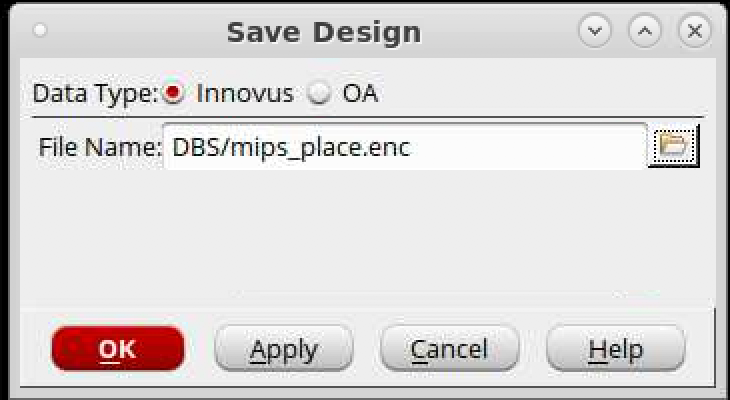
\includegraphics[scale=0.35]{figures/lab5_backend/save_design}
			\caption{Saving your design.}
			\label{fig_save_design}
		\end{wrapfigure}
	To save the current design:
		\vspace{-4mm}
		\item Go to \textit{File -> Save Design...}
		\item Select the \textit{Innovus} Data Type as shown in Fig. \ref{fig_save_design} and specify the file name \textit{mips$\_$nameofstep.enc}
		\item Click on \textit{OK}.  \\ 
		Equivalent Innovus command:
		\begin{codeline}
			saveDesign DBS/mips$\_$nameofstep.enc
		\end{codeline}
		
	}
\end{enumerate}


		\vspace{-9mm}
\begin{remark}
	When saving your design after each step, do not forget to change the name of the file (for instance, \textit{mips$\_$place.enc} after the placement step).
\end{remark}

\begin{enumerate}
	\parbox[t]{\dimexpr\textwidth-\leftmargin}{%

		\begin{wrapfigure}[10]{r}{0.45\textwidth}
					\vspace{0mm}
			\centering
			\vspace{-\baselineskip}
			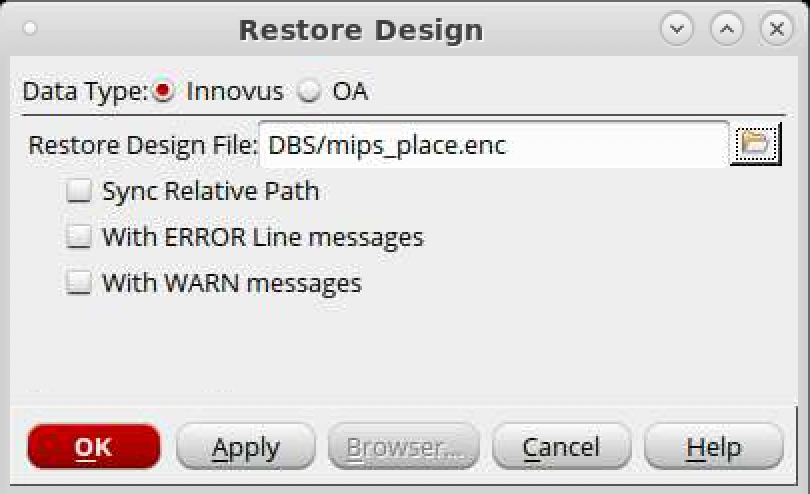
\includegraphics[scale=0.35]{figures/lab5_backend/restore_design}
		\caption{Restoring a previous design.}
			\label{fig_restore_design}
		\end{wrapfigure}
	To restore a previous design:
			\vspace{-4mm}
		\item Go to \textit{File -> Restore Design...}
	\item Select the \textit{DB/Processor$\_$nameofstep.enc} file to restore as depicted in Fig. \ref{fig_restore_design}.
		\item Click on \textit{OK}.  \\
		Equivalent Innovus command:
		\begin{codeline}
			restoreDesign DBS/mips$\_$nameofstep.enc mips
		\end{codeline}
	} 
\end{enumerate}



\newpage
\subsection{Floorplanning the Design}
In this step, you will define the \textit{core area} of your design, where the logic cells from your gate-level netlist from synthesis will be placed. You can define the aspect ratio, the form of the core, the distance between the core and the pads \textit{etc.}. After the design import, a default floorplan is shown in the display area. 
\subsubsection{Defining the Floorplan Settings}
To specify the floorplan:
\begin{enumerate}
	\parbox[t]{\dimexpr\textwidth-\leftmargin}{%		
		\begin{wrapfigure}[20]{r}{0.45\textwidth}
			\vspace{-15mm}
			\centering
			\vspace{-\baselineskip}
			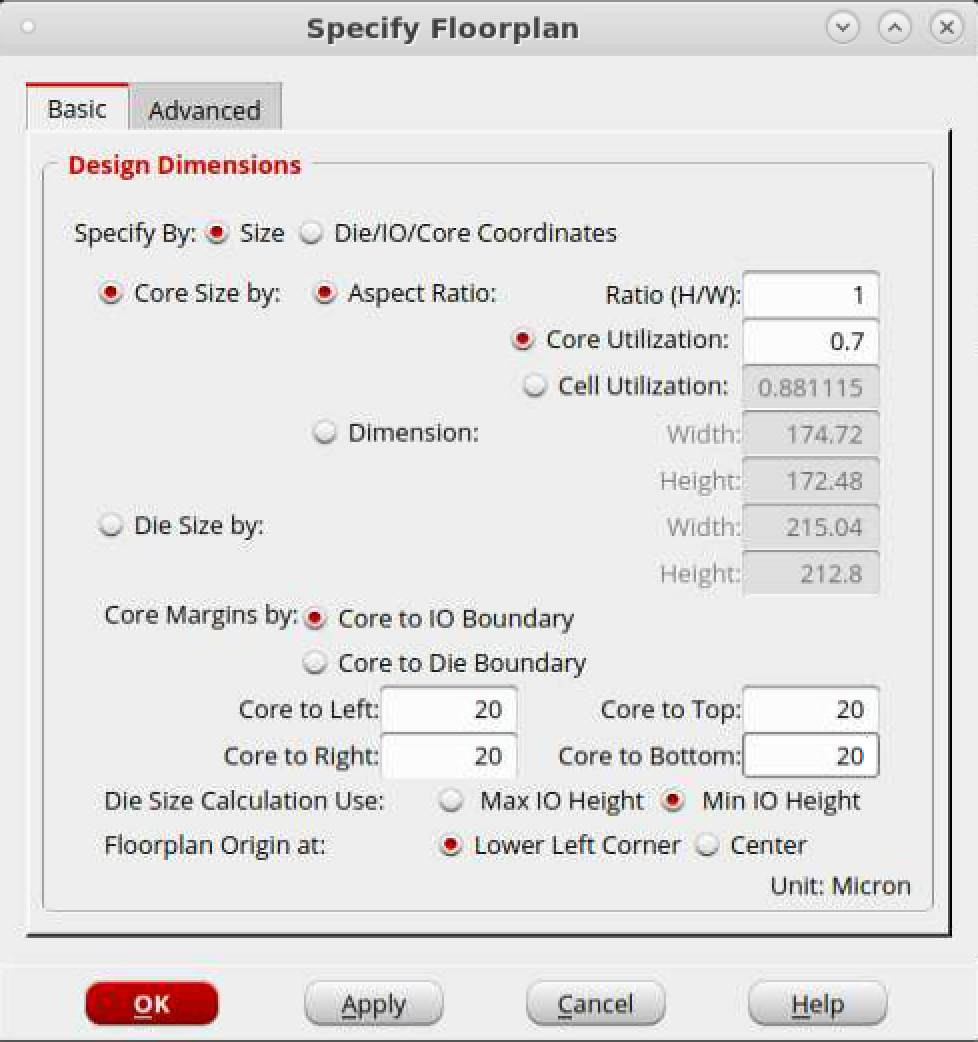
\includegraphics[scale=0.4]{figures/lab5_backend/floorplan}
			\caption{Specifying the floorplan.}
			\label{fig_floorplan}
		\end{wrapfigure}
		\item Go to \textit{Floorplan-> Specify Floorplan...}
		\item Define the settings as in Fig. \ref{fig_floorplan}. \\ The \textit{Aspect ratio (H/W)}: means that your core area will have a square form. \\ \textit{Core Utilization}: 70$\%$ of the core area will be used for placing the standard cells and the 20$\%$ remaining will be free for power routing, buffer insertion etc. \\ \textit{Core Margins}: means that the distance between the core area to the core bounding box will be 20 $\mu$$m$. 
		\item Click on \textit{OK}.  \\ \\
		Equivalent Innovus command:
		\begin{codeline}
			floorPlan -site core7T -r 1 0.7 20 20 20 20
		\end{codeline}
	}
\end{enumerate}

 Before going any further, a setting has to be made in order for you to be able to display all the verilog modules on your floorplan, even the ones with a small size. To do so:
 \begin{enumerate}
 	\item \textit{View -> Set Preferences...}.
 	\item Select the \textit{Display} tab.
 	\item Next to the \textit{Min. Floorplan Module Size}, replace 100 by 1.
 	\item Click Ok.
 \end{enumerate}
Equivalent Innovus command:
\begin{codeline}
setPreference MinFPModuleSize 1
\end{codeline}


 Now, you can look at the floorplan overall organization. Select the \textit{Floorplan view icon} \img{figures/lab5_backend/fp_icon} to display all the modules and blocks, as illustrated in Fig. \ref{floorplan_view}. The objects on the left are the \textcolor{blue}{\textbf{modules}} from your Verilog netlist. They can be moved and reshaped. The objects on the right of the core area are unplaced \textcolor{blue}{\textbf{blocks}} that can only be moved (since their physical design is already defined by the IP provider). Those are generally the IP components such as an RF macro or an SRAM array. Select the \textit{dp} module on the left, and press \textbf{shift+g}. You just now descended in its hierarchy and can observe the verilog modules it contains. This can be done for all the hierarchical levels. To revert this action and only display the higher module in terms of hierarchy, select the appropriate module and press \textbf{g}. \newline
 
 Each module shows a target utilization (TU) value that represents its physical design size. Left-clicking on a module or a block displays the pins and connection flight lines, which are the connections and number of connections between the selected module or block to any other modules and blocks.



	\begin{figure}[!h]
	\centering
	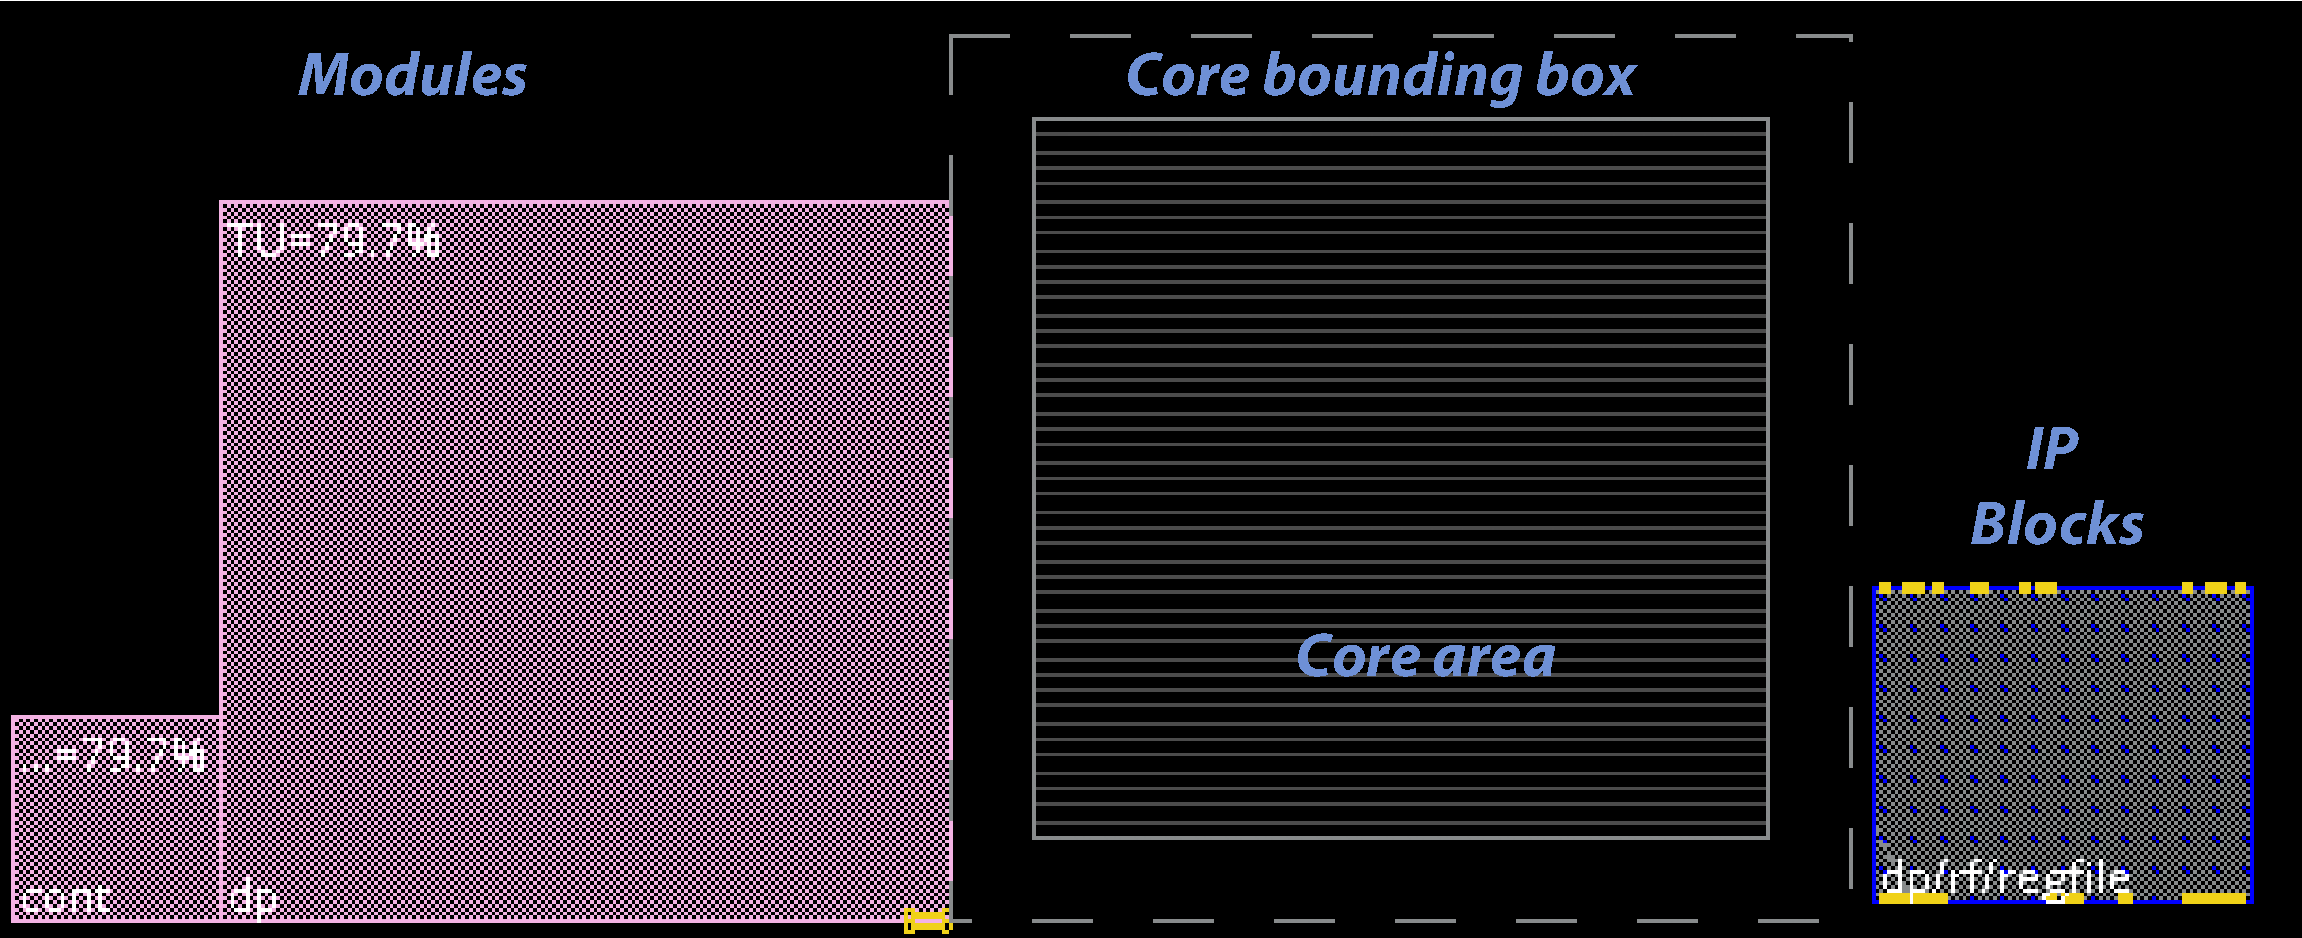
\includegraphics[scale=0.43]{figures/lab5_backend/floorplan_view.pdf}
	\caption{Floorplan View.}
	\label{floorplan_view}
\end{figure}

%\clearpage
\subsubsection{Placing the Register Block}
In large designs, the cache or registers of your processor are generally provided as an IP block (or hard macro) whose layout and internal timing are already defined. In this lab, the \textit{mips} processor uses a small 8$\times$8 register, which is the IP block you can see on the right side of the floorplan view. To place the register IP:
\begin{enumerate}
	\parbox[t]{\dimexpr\textwidth-\leftmargin}{%		
		\begin{wrapfigure}[20]{r}{0.45\textwidth}
			\vspace{0mm}
			\centering
			\vspace{-\baselineskip}
			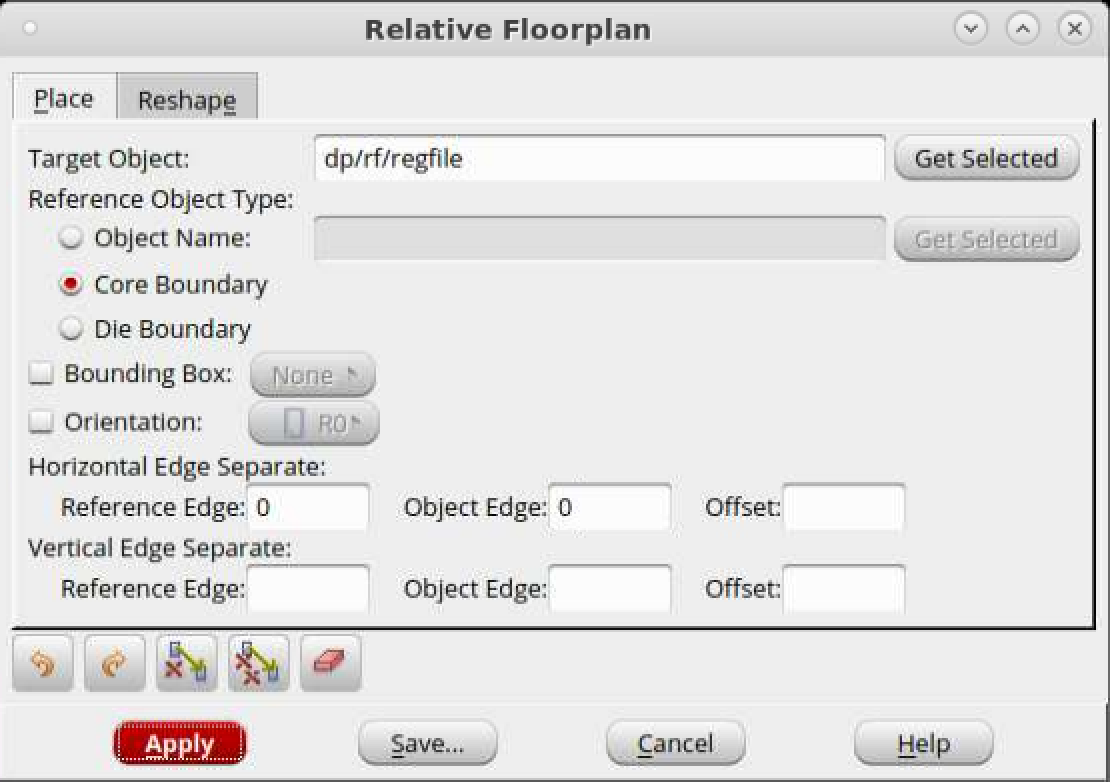
\includegraphics[scale=0.32]{figures/lab5_backend/place_reg}
			\caption{Placing the register module.}
			\label{place_reg}
		\end{wrapfigure}
	    \item Select the register IP by left clicking on it.
		\item Go to \textit{Floorplan-> Relative Floorplan -> Edit Constraints...}
		\item Define the settings as in Fig. \ref{place_reg}. It will place the register module on the left side of the core area, aligned with the bottom side.
		\item Click on \textit{Apply}. The register module is now placed. Close the window.
	}

\end{enumerate}
Equivalent Innovus command:
\begin{codeline}
create$\_$relative$\_$floorplan -place dp/rf/regfile -ref$\_$type core$\_$boundary\\
-horizontal$\_$edge$\_$separate $\{$0  ""  0$\}$ -vertical$\_$edge$\_$separate $\{$"" "" ""$\}$
\end{codeline}

Then, a placement halo around the register IP block has to be defined. It will prevent standard cells to be placed too closely to the block. Also, since there will be power rings around the block, this will ensure that the power rails of the standard cells are properly connect to the block power rings (see Section \ref{power}). To do so:

\begin{enumerate}
	\parbox[t]{\dimexpr\textwidth-\leftmargin}{%		
		\begin{wrapfigure}[20]{r}{0.45\textwidth}
			\vspace{-3mm}
			\centering
			\vspace{-\baselineskip}
			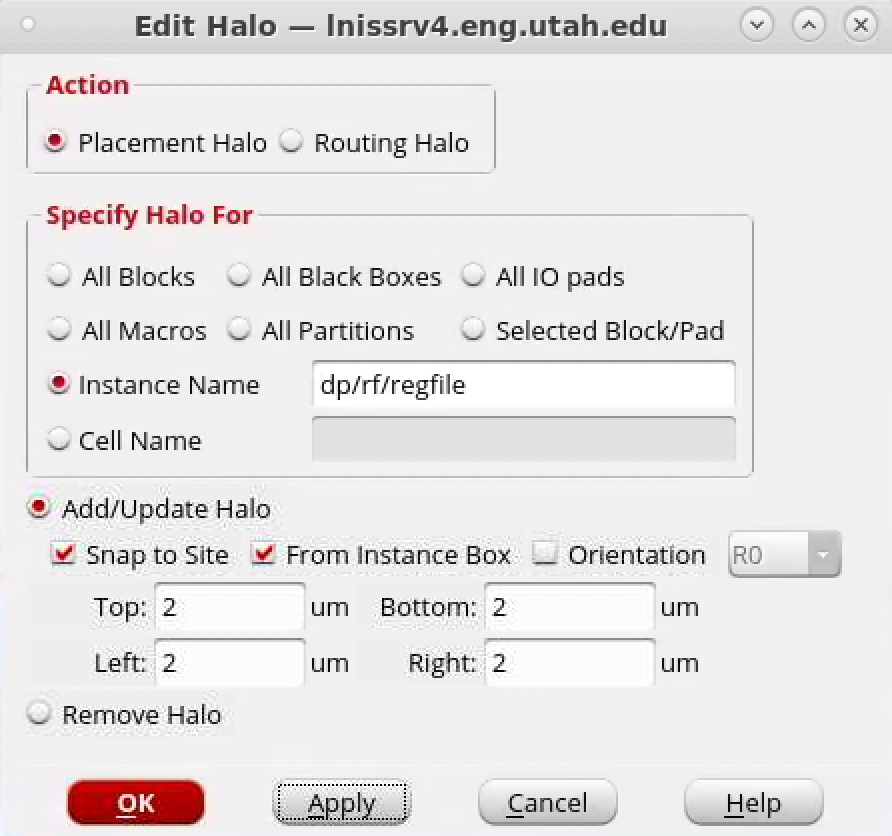
\includegraphics[scale=0.32]{figures/lab5_backend/halo_reg}
			\caption{Adding a placement halo around the register block.}
			\label{halo_reg}
		\end{wrapfigure}
		\item Right click on the register IP block and go to: \textit{Edit Halo...}.
\item Define the settings as in Fig. \ref{halo_reg}. It will add a placement halo on each sides of 2 $\mu$$m$. Note that the \textit{Snap to Site} option was selected, so the Halo is rounded up to the nearest site, so the enarest standard cell row. In P\&R, a SITE has a SIZE which is the base area that the SITE occupies. A macro or a standard cell sit on a SITE, and its size must match or be an integral multipliers of the base SITE. In this lab, you are using a SITE of size 0.560 $\times$ 3.920, meaning that each standard cell has a height of 3.920 $\mu m$ and a width of a multiple of 0.560 $\mu m$.

\item Click on \textit{OK}.
	}
\end{enumerate}
			\vspace{20mm}
Equivalent Innovus command:
\begin{codeline}
addHaloToBlock {2 2 2 2} -fromInstBox -snapToSite dp/rf/regfile
\end{codeline}

Before going any further, you can notice that some gap between the register IP and the core boundary. This is because the register file has some integrated power rings. To display those, in the \textit{Visibility Toggles} on the right side, expend \textit{Cell} and check \textit{Pin Shapes} and uncheck \textit{Cell Blockage}, as shown in Fig. \ref{toggles}. You can now observe the power rings around the IP block.

	\begin{figure}[!h]
	\centering
	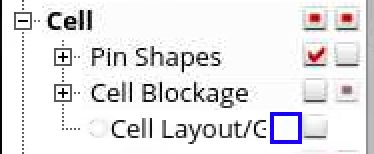
\includegraphics[scale=0.43]{figures/lab5_backend/halo_view}
	\caption{Visibility toggles for the IP block.}
	\label{toggles}
\end{figure}
\clearpage

\subsection{Defining the Power Structure}\label{power}
This step will define the power structure of the chip, such as the power rings and the power stripes around the core and will also route all the power nets. 

\subsubsection{Logically Connecting all the Power/Ground Nets}
The netlist does not include any power and ground connection but the cells that will be placed do have power and ground connections. Therefore, you need to logically connect all the power nets of the cells to the global power net you defined during the import phase ($V_{DD}$ and $V_{SS}$). 


	\parbox[t]{\dimexpr\textwidth-\leftmargin}{%		
		\begin{wrapfigure}[40]{r}{0.36\textwidth}
			\vspace{0mm}
			\centering
			\vspace{-\baselineskip}
			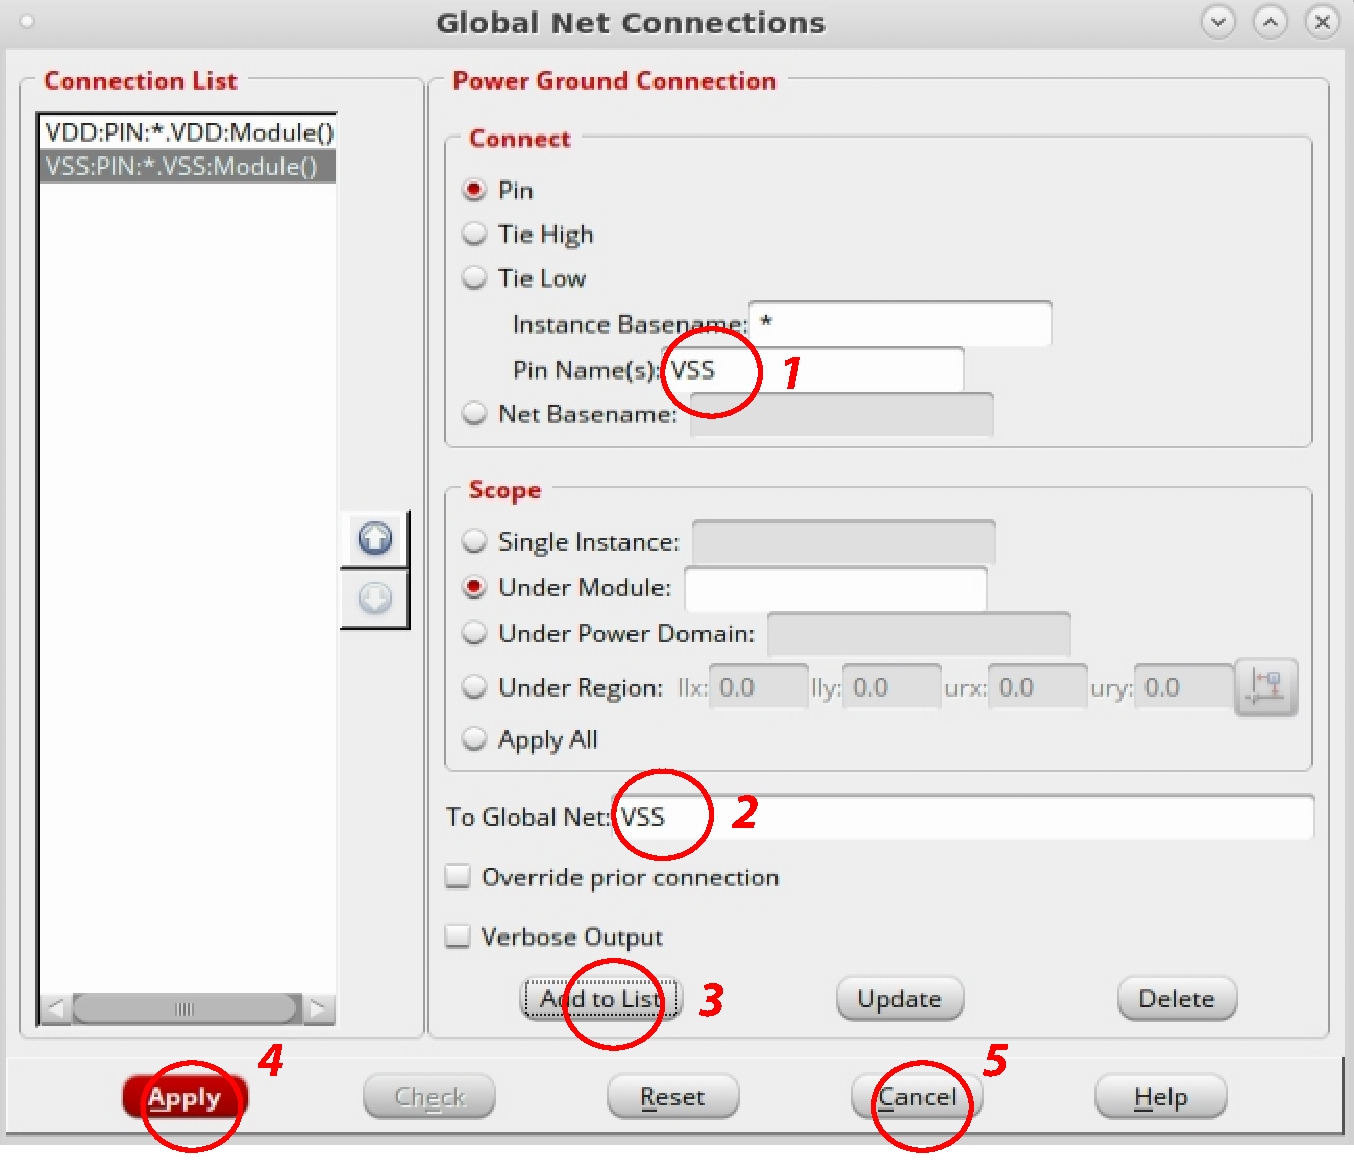
\includegraphics[scale=0.28]{figures/lab5_backend/powernet.pdf}
			\caption{Connecting the power nets.}
			\label{fig_powernets}
		\end{wrapfigure}
	To do so:
	\begin{enumerate}
		\item Go to \textit{Power->  Connect Global Nets...}
		\item For each global net ($V_{DD}$ and $V_{SS}$), do as in Fig. \ref{fig_powernets}.
		\item Click on \textit{OK} then \textit{Cancel}.

\end{enumerate}
Equivalent Innovus command:
\begin{codeline}
globalNetConnect VDD -type pgpin -pin VDD $\textbackslash$ \\-instanceBasename * -hierarchicalInstance $\{\}$ \\
globalNetConnect VSS -type pgpin -pin VSS  $\textbackslash$ \\ -instanceBasename *-hierarchicalInstance $\{\}$ 
\end{codeline}
	} 
			\vspace{8mm}

\subsubsection{Adding the Power Rings Around the Core}
Now that the power and ground nets are logically assigned, power planning can be done. First, lets add the power ring around the core area.
\begin{enumerate}
	\parbox[t]{\dimexpr\textwidth-\leftmargin}{%		
		\begin{wrapfigure}[20]{r}{0.5\textwidth}
			\vspace{-10mm}
			\centering
			\vspace{-\baselineskip}
		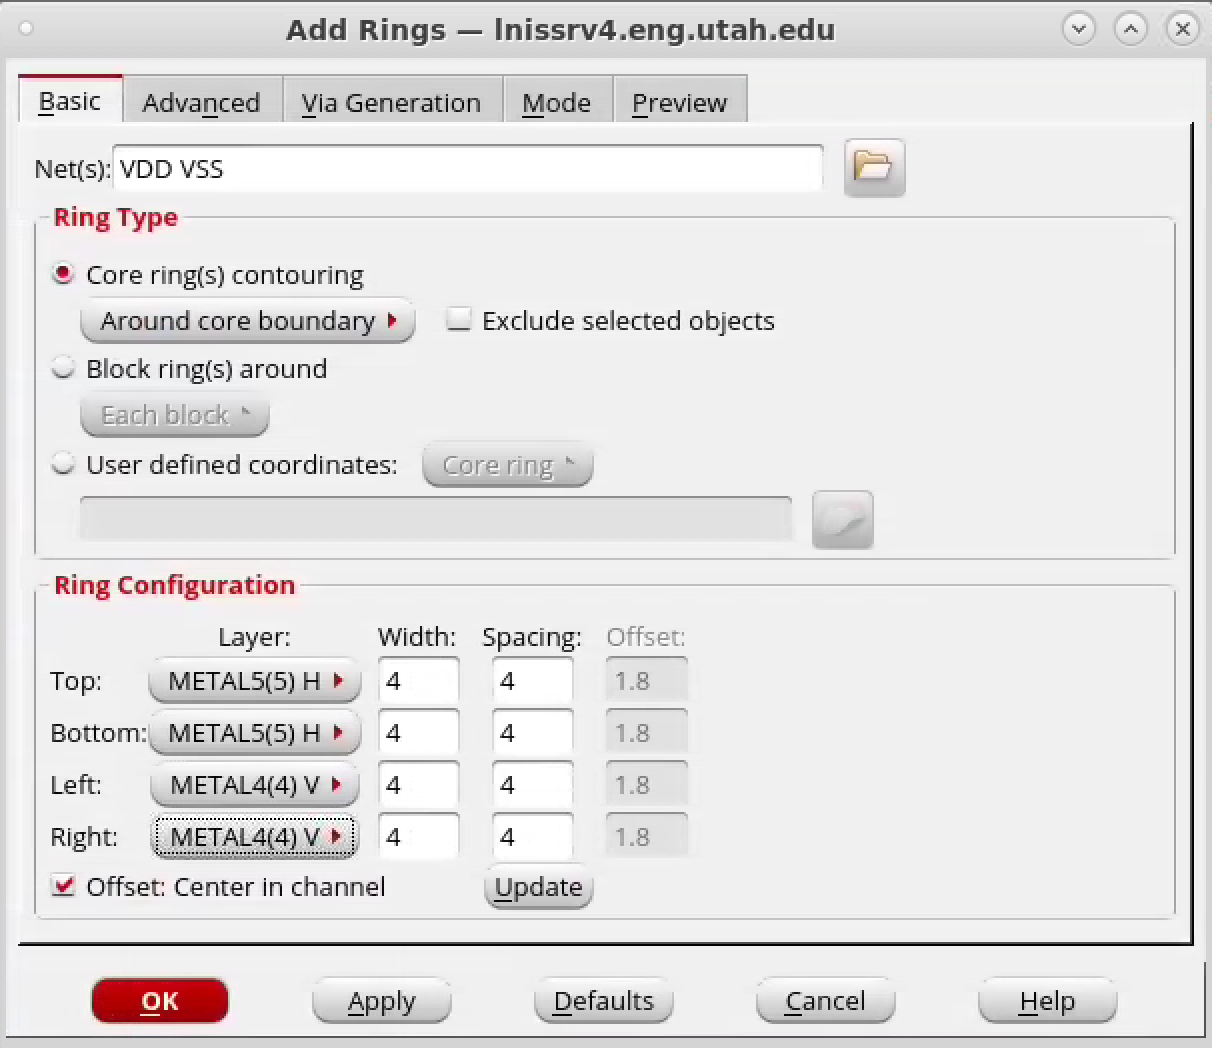
\includegraphics[scale=0.35]{figures/lab5_backend/addring}
\caption{Adding the power ring around the core area.}
			\label{fig_addring}
		\end{wrapfigure}
	\item Go to \textit{Power -> Power Planning -> Add Ring...}
\item Specify the power and ground nets as in Fig. \ref{fig_addring}.
\item Specify the layers and the width of each ring as well as the spacing between each ring, as in Fig. \ref{fig_addring}. The \textit{Ring Configuration} defines the ring metal wires widths and spacing. Here, the horizontal power metal wires will be in metal5 and the vertical ones in metal4. The ring will be placed in the center of the channel between the core and the chip boundary (or the I/O pads, if there are some).
\item Click on \textit{OK}.	
	}
\end{enumerate}
Equivalent Innovus command:
\begin{codeline}
addRing -nets $\{$VDD VSS$\}$ -type core$\_$rings -follow core -layer $\textbackslash$ \\$\{$top METAL5 bottom METAL5 left METAL4 right METAL4$\}$ -width $\textbackslash$ \\$\{$top 4 bottom 4 left 4 right 4$\}$ -spacing $\textbackslash$ \\$\{$top 4 bottom 4 left 4 right 4$\}$ -offset $\textbackslash$ \\$\{$top 1.8 bottom 1.8 left 1.8 right 1.8$\}$ -center 1 -extend$\_$corner $\{$ $\}$$\textbackslash$ \\ -threshold 0 -jog$\_$distance 0 -snap$\_$wire$\_$center$\_$to$\_$grid None
\end{codeline}

\begin{exercise}
Which metal layers should be used for power routing and for the CTS and why (it is not necessarily the default one used in this lab)?
\end{exercise}



\subsubsection{Adding Power Stripes}
Power stripes are vertical or horizontal power lines spanning across the core area. They can be needed to ensure the proper power distribution in large cores to avoid IR drop. To do so:


\begin{enumerate}
	\parbox[t]{\dimexpr\textwidth-\leftmargin}{%		
		\begin{wrapfigure}[20]{r}{0.5\textwidth}
			\vspace{0mm}
			\centering
			\vspace{-\baselineskip}
			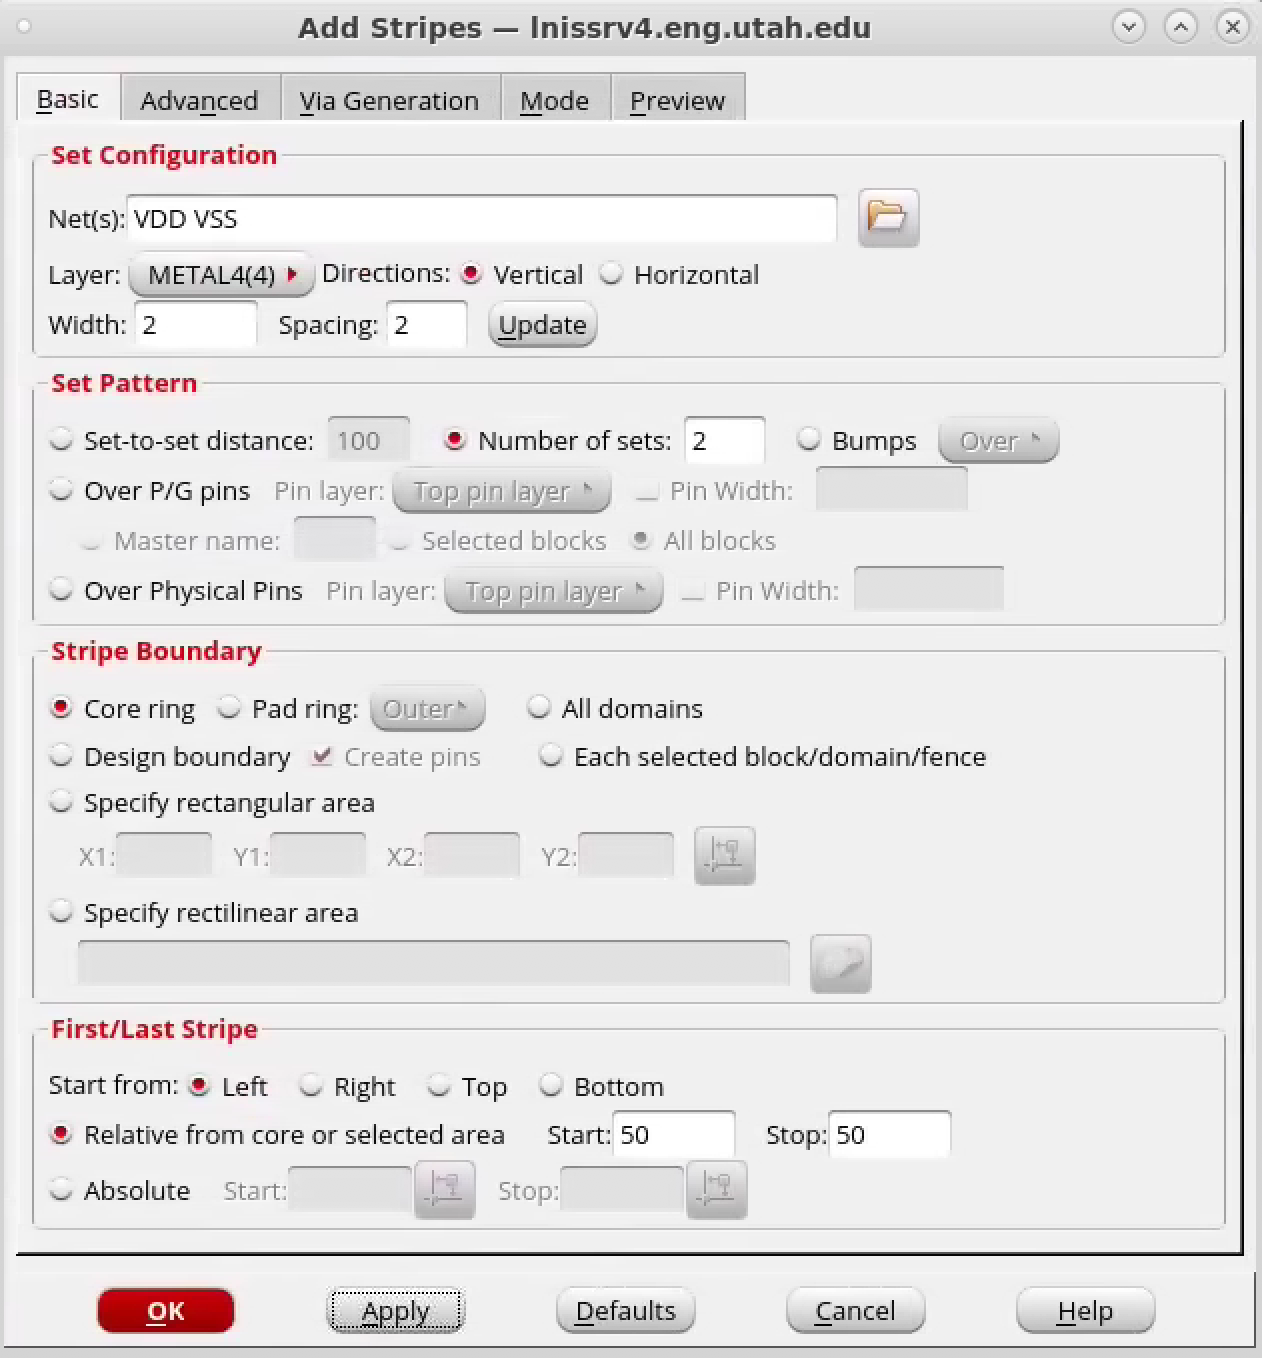
\includegraphics[scale=0.4]{figures/lab5_backend/add_stripes}
			\caption{Adding Power Stripes.}
			\label{add_stripes}
		\end{wrapfigure}
	\item Go to \textit{Power -> Power Planning -> Add Stripes...}
\item Define the settings as in Fig. \ref{add_stripes}. It will create 2 pairs of $VDD$ and $VSS$ power stripes in metal4, starting and ending 50 $\mu$$m$ of the left and right sides. 
	\item Click on \textit{OK}.	You can now see the vertical power stripes on the floorplan.
	} 
\end{enumerate}
\vspace{170px}
Equivalent Innovus command:
\begin{codeline}
addStripe -nets {VDD VSS} -layer METAL4 -direction vertical -width 2 -spacing 2 -number$\_$of$\_$sets 2 -start$\_$from left -start$\_$offset 50 -stop$\_$offset 50 -switch$\_$layer$\_$over$\_$obs false -max$\_$same$\_$layer$\_$jog$\_$length 2 -padcore$\_$ring$\_$top$\_$layer$\_$limit METAL6 -padcore$\_$ring$\_$bottom$\_$layer$\_$limit METAL1 -block$\_$ring$\_$top$\_$layer$\_$limit METAL6 -block$\_$ring$\_$bottom$\_$layer$\_$limit METAL1 -use$\_$wire$\_$group 0 -snap$\_$wire$\_$center$\_$to$\_$grid None
\end{codeline}


\clearpage

\subsubsection{Routing the Power Nets}
\begin{enumerate}
	\parbox[t]{\dimexpr\textwidth-\leftmargin}{%		
		\begin{wrapfigure}[20]{r}{0.5\textwidth}
			\vspace{0mm}
			\centering
			\vspace{-\baselineskip}
			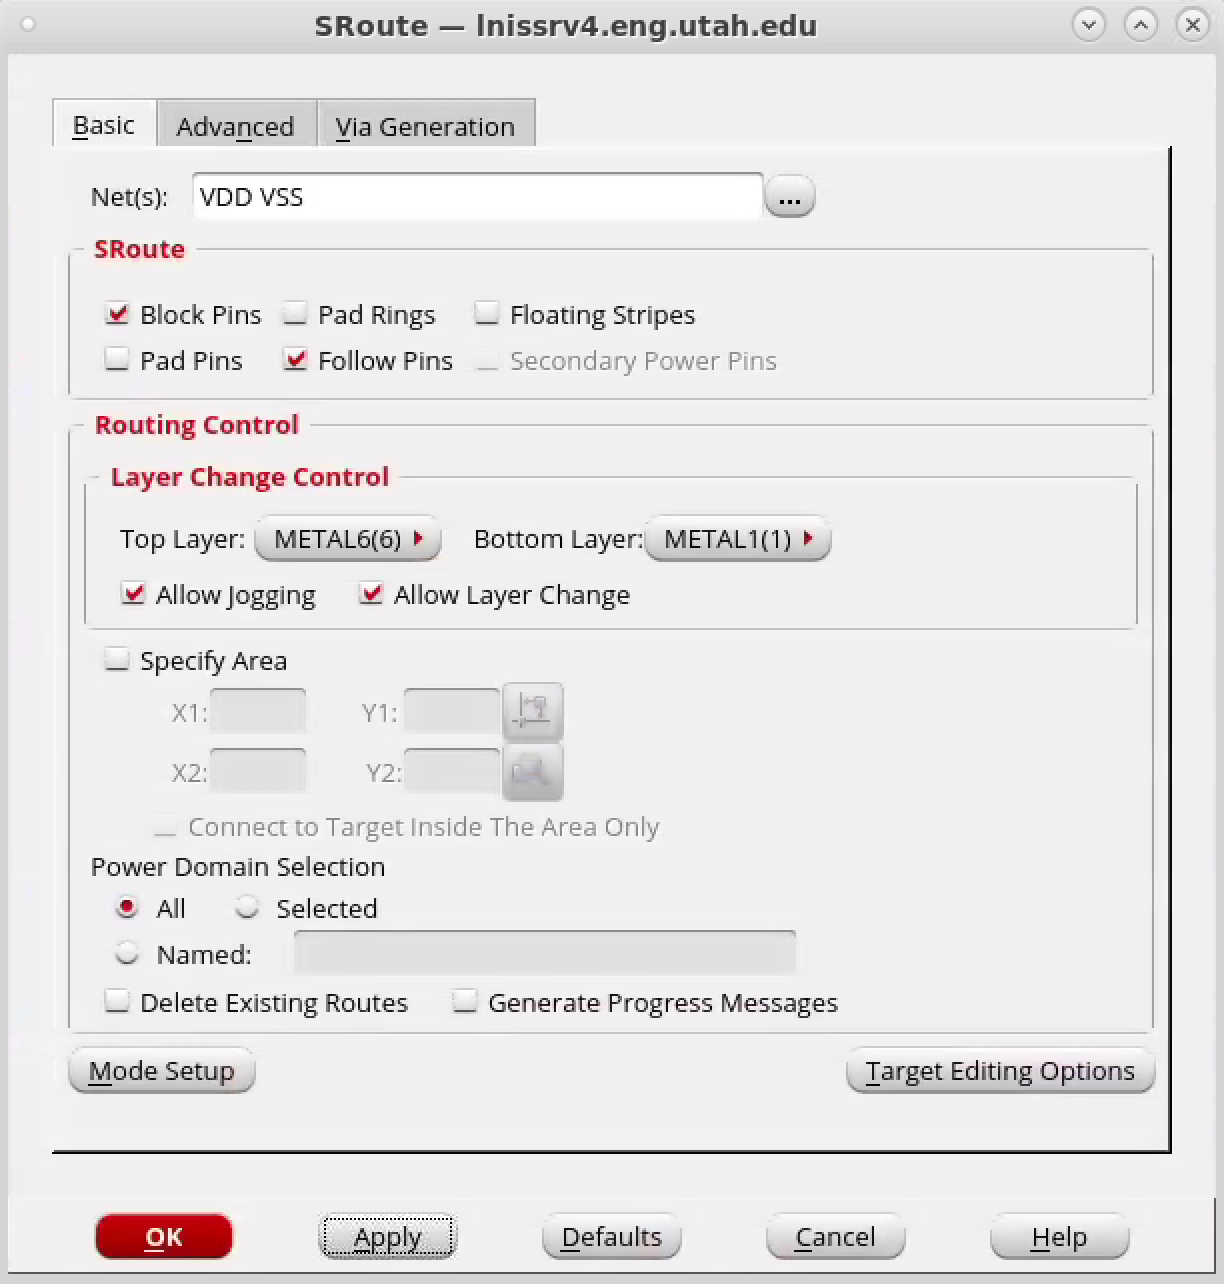
\includegraphics[scale=0.45]{figures/lab5_backend/routesc_options}
			\caption{Routing the power nets.}
			\label{fig_specialroute}
		\end{wrapfigure}
	Now, the power net can be routed. This step will create the vertical $V_{DD}$ and $V_{SS}$ power lines on the entire core area. This is why it is important, when designing full custom cells (as you did in the previous labs), to use the same height for each of your cells so they fit between those power lines.
		\item Go to \textit{Route -> Special Route...}
		\item In the \textit{Basic} tab, specify the power net name as shown in Fig. \ref{fig_specialroute}. Only check the \textit{Block Pins} and \textit{Follow Pins} boxes.
		\item Click on \textit{OK}.	You can now see the horizontal power lines on the floorplan.
	} 
\end{enumerate}
			\vspace{24mm}
Equivalent Innovus command:
\begin{codeline}
sroute -connect $\{$blockPin corePin$\}$ -layerChangeRange $\{$METAL1(1) METAL6(6)$\}$ $\textbackslash$ \\-blockPinTarget $\{$ nearestTarget $\}$ -corePinTarget $\{$ firstAfterRowEnd $\}$ $\textbackslash$\\ -allowJogging 1 -crossoverViaLayerRange $\{$METAL1(1) METAL6(6)$\}$ $\textbackslash$ \\-nets $\{$ VDD VSS $\}$ -allowLayerChange 1 -blockPin useLef $\textbackslash$ \\-targetViaLayerRange $\{$METAL1(1) METAL6(6)$\}$
\end{codeline}


%Now, the power step is done. Save your design as \textit{DBS/mips$\_$power.enc}, as explained in Section \ref{save}. 

	\parbox[t]{\dimexpr\textwidth-\leftmargin}{%		
	\begin{wrapfigure}[20]{r}{0.3\textwidth}
		\vspace{0mm}
		\centering
		\vspace{-\baselineskip}
	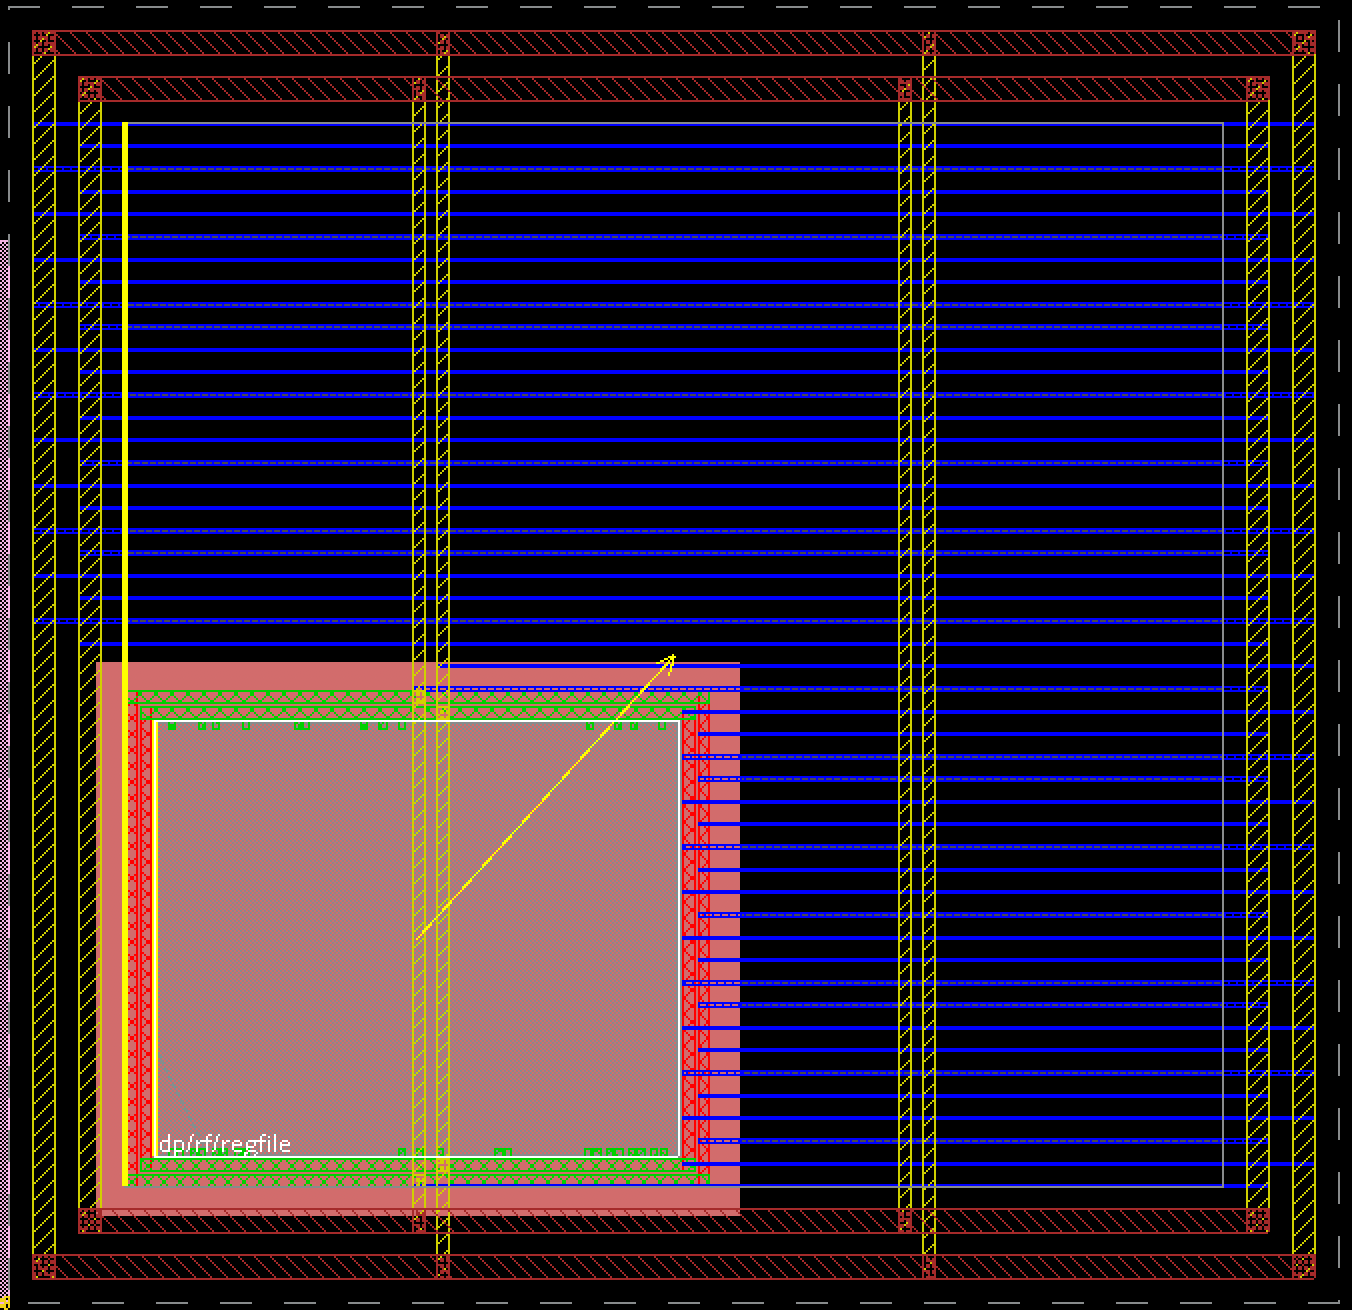
\includegraphics[scale=0.3]{figures/lab5_backend/mips_floorplan}
\caption{Design after the floorplaning step.}
\label{mips_floorplan}
	\end{wrapfigure}
The floorplan of your design is done. It should looks like Fig. \ref{mips_floorplan}. Save your design as \textit{DBS/mips$\_$fplan$\_$power.enc}, as explained in Section \ref{save}. For more complex design, the floorplanning is generally the most important step since many particular modules (such as IP, RF modules or caches) have to be placed, requiring many halo for routing and placement, special power rings and stripes, \textit{etc.}
				\begin{codeline}
	saveDesign DBS/mips$\_$fplan$\_$power.en
\end{codeline}

\begin{checkpoint}\label{check1}
	Please call an assistant and show him that your floorplan looks correct.
\end{checkpoint}
}
\clearpage

\subsection{Placing the Standard Cells}
This step will place the standard cells (contained in your Verilog netlist) in the floorplan rows.
\begin{enumerate}
	\parbox[t]{\dimexpr\textwidth-\leftmargin}{%		
		\begin{wrapfigure}[20]{r}{0.\textwidth}
			\vspace{-14mm}
			\centering
			\vspace{-\baselineskip}
	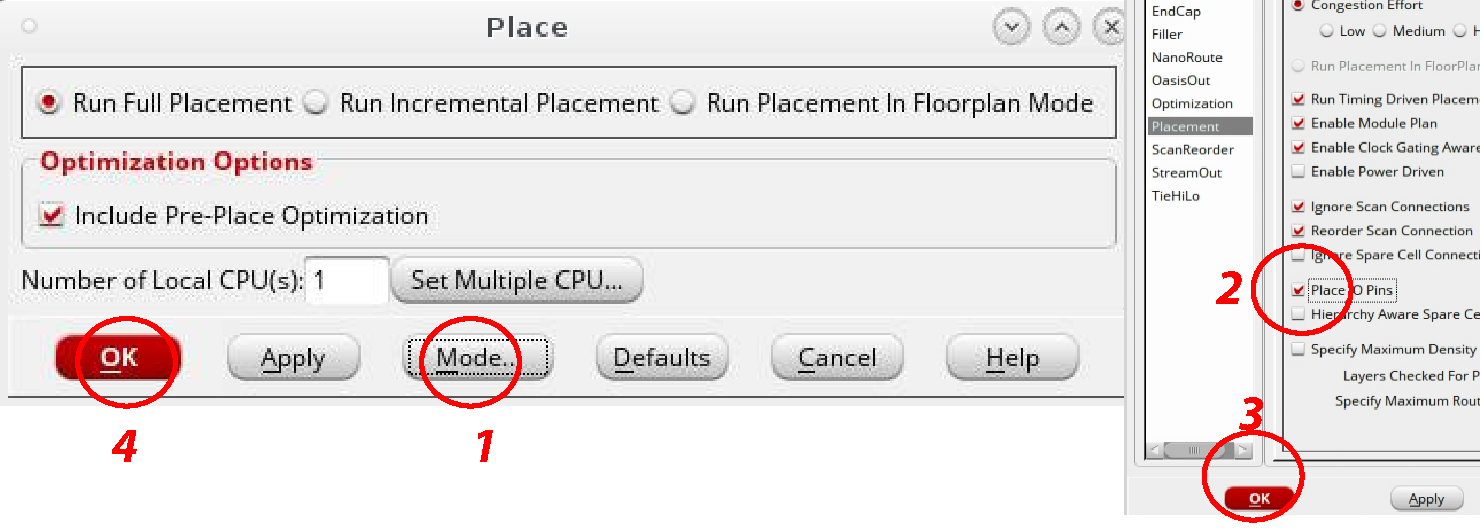
\includegraphics[scale=0.4]{figures/lab5_backend/place.pdf}
\caption{Placement settings.}
\label{fig_place}
		\end{wrapfigure}
\item Go to \textit{Place -> Place standard Cells...}
\item Click on \textit{Mode...}.
\item In the \textit{Placement} tab, select \textit{Place IO pins}, as shown in Fig. \ref{fig_place}.
\item Click on \textit{Ok} then on \textit{Ok}.
	} \\ \\ \\ 
\end{enumerate}

Equivalent Innovus command:
\begin{codeline}
setPlaceMode -placeIOPins 1 \\
place$\_$design
\end{codeline}




	\parbox[t]{\dimexpr\textwidth-\leftmargin}{%		
		\begin{wrapfigure}[18]{r}{0.45\textwidth}
			\vspace{0mm}
			\centering
			\vspace{-\baselineskip}
			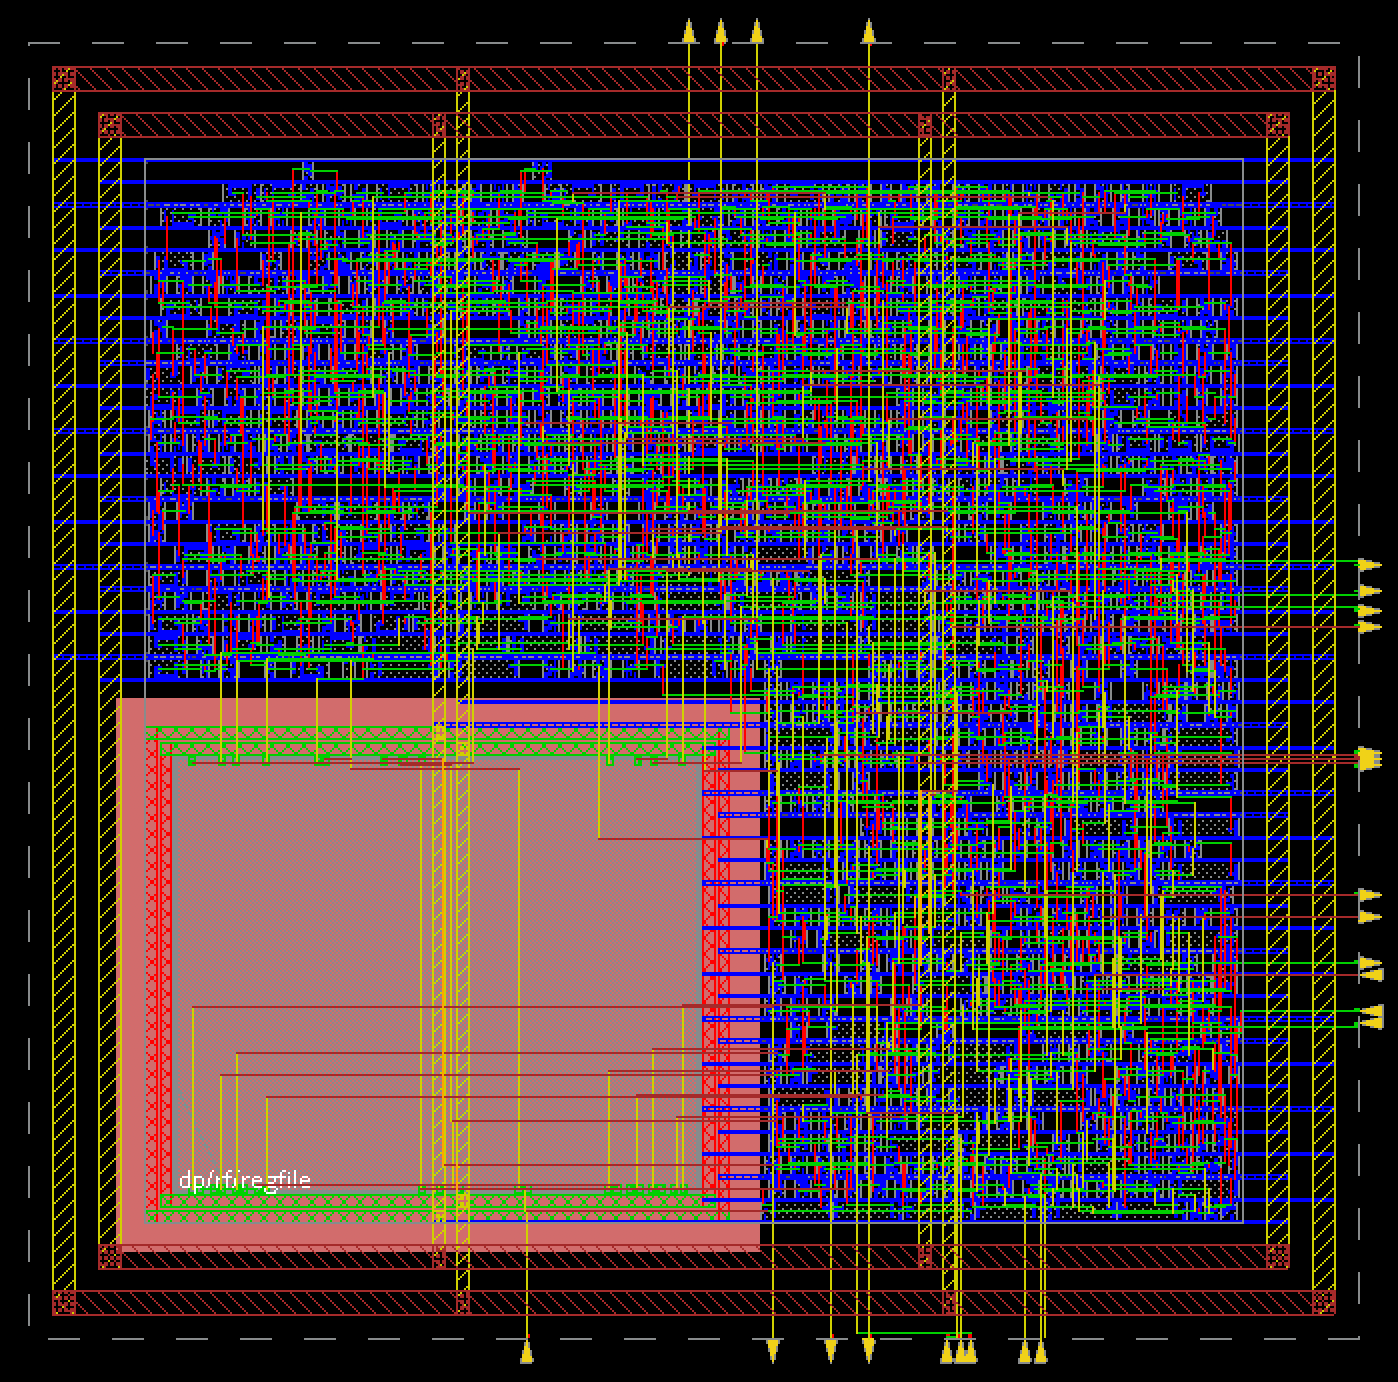
\includegraphics[scale=0.27]{figures/lab5_backend/design_placed}
			\caption{Placed design.}
			\label{fig_place_design}
		\end{wrapfigure}
Select the Physical view icon \img{figures/lab5_backend/physical_view} to see the result of the placement in the display area. It should look something like Fig. \ref{fig_place_design} The placement has been ran in \textit{Timing-Driven mode}. That means the Placement program balances the importance of meeting setup timing constraints (from the \textit{.sdc} file) with routability. This is why you can see routing wires. However, those are not the final ones. The final ones will be obtained after the Routing step. \\
As you can see, some rows have holes. This is because you specified a core utilization of 80$\%$ when defining the floorplan properties. This space will be filled by buffers or inverters (for the clock tree). Some cells will also be replaced (by the same cell but with a higher driving capability) when performing timing-driven optimization in the next steps. \\
	} 

After the placement step, you can obtain some information about the design:
\begin{enumerate}
	\parbox[t]{\dimexpr\textwidth-\leftmargin}{%		
		\begin{wrapfigure}[20]{r}{0.4\textwidth}
			\vspace{0mm}
			\centering
			\vspace{-\baselineskip}
			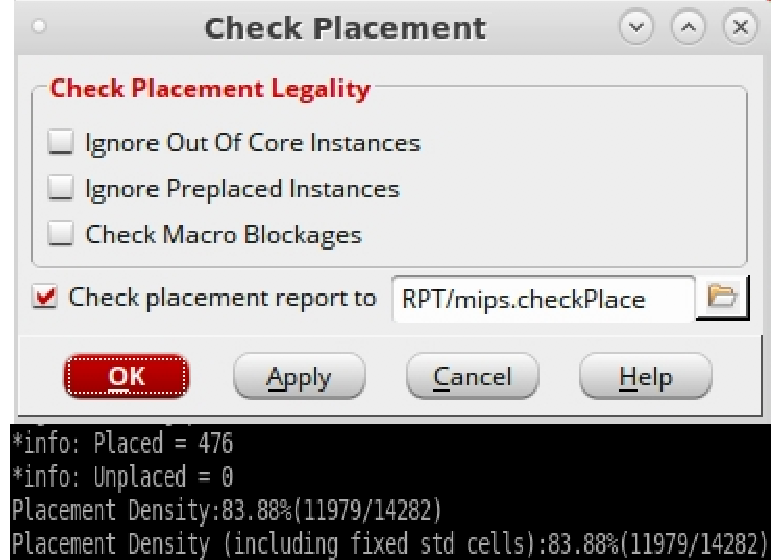
\includegraphics[scale=0.45]{figures/lab5_backend/checkplace.pdf}
			\caption{Checking the placement.}
			\label{checkplace}
		\end{wrapfigure}
		\item Go to \textit{Place -> Check Placement...}.
		\item You can check or not the \textit{Check Placement report to} if you want to keep the report in a file (the recommended
location is then in the file \textit{RPT/mips.Checkplace.rpt}.
		\item Click on \textit{Ok}. You can now see the density of your design (which should be close to 80$\%$), the number of placed cells, \textit{etc.} \\ 
		Equivalent Innovus command:
		\begin{codeline}
			checkPlace RPT/mips.checkPlace.rpt
		\end{codeline}
		
	} 
\end{enumerate}



After the placement step, you can obtain a first estimation of the critical path. This is only an estimation since the routing step has not been completed yet. To do so:
\begin{enumerate}
	\parbox[t]{\dimexpr\textwidth-\leftmargin}{%		
		\begin{wrapfigure}[20]{r}{0.45\textwidth}
			\vspace{-5mm}
			\centering
			\vspace{-\baselineskip}
			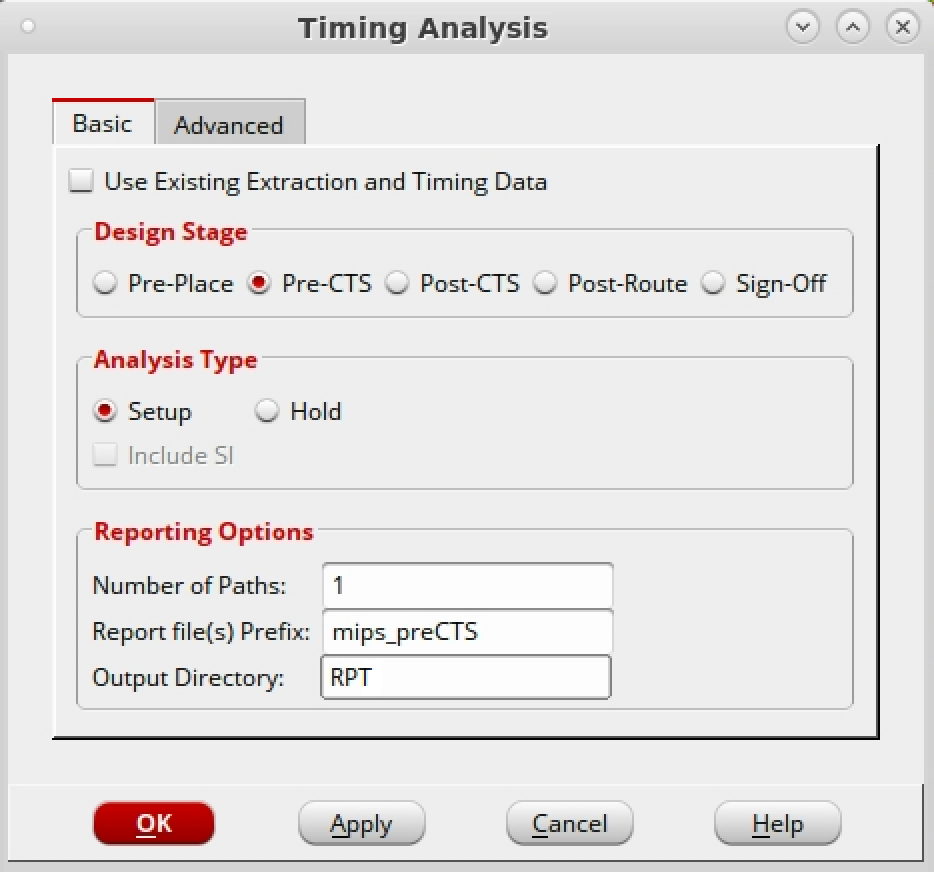
\includegraphics[scale=0.38]{figures/lab5_backend/report_timing_ino}
			\caption{Timing analysis settings.}
			\label{fig_timing}
		\end{wrapfigure}
	\item The first step is to tell Innovus\textsuperscript{\tiny\textregistered} which technology node you are using. It will ensure better accuracy results when extracting the timing delay. In the terminal, write:
			\begin{codeline}
		setDesignMode ‐process 180
	\end{codeline}
		\item Go to \textit{Timing -> Report Timing...}
		\item Keep the same settings as depicted in Fig. \ref{fig_timing}. Especially, keep the \textit{Pre-CTS} box checked since we want to get the timing before the \textit{CTS} step.
		\item Click on \textit{Ok}.
	} \\ 
\end{enumerate}
Equivalent Innovus command:
		\begin{codeline}
timeDesign -preCTS -pathReports -drvReports -slackReports -numPaths 1 $\textbackslash$\\-prefix mips$\_$preCTS -outDir RPT
		\end{codeline}

	\parbox[t]{\dimexpr\textwidth-\leftmargin}{%		
	\begin{wrapfigure}[10]{r}{0.55\textwidth}
		\vspace{0mm}
		\centering
		\vspace{-\baselineskip}
	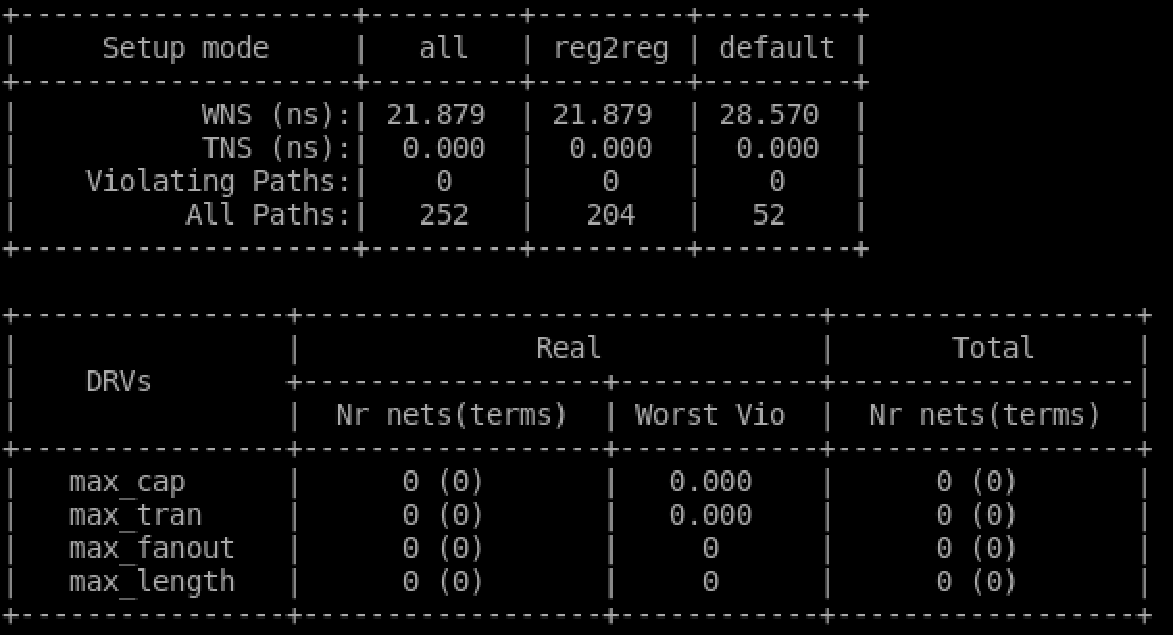
\includegraphics[scale=0.4]{figures/lab5_backend/timing_prects.pdf}
\caption{Pre-CTS slack report.}
\label{fig_timing_prects}
	\end{wrapfigure}
On the console terminal, you can now see some timing information, as sown in Fig. \ref{fig_timing_prects}. The \textit{Worst Negative Slack} (WNS) is the slack of the critical path in the design. Here, it has a positive value so the timing constraints are already met. Even if it had a negative value, the slack could still become positive after the next optimization step. On the \textit{DRC} table, you might see a few violations such as \textit{max$\_$cap, max$\_$tran, etc.}. Those can be resolved by optimizing your design.\\
} 

		\vspace{4mm}
To optimize your design after the place step:
		\vspace{-2mm}
\begin{enumerate}
	\parbox[t]{\dimexpr\textwidth-\leftmargin}{%		
		\begin{wrapfigure}[20]{r}{0.4\textwidth}
			\vspace{-10mm}
			\centering
			\vspace{-\baselineskip}
			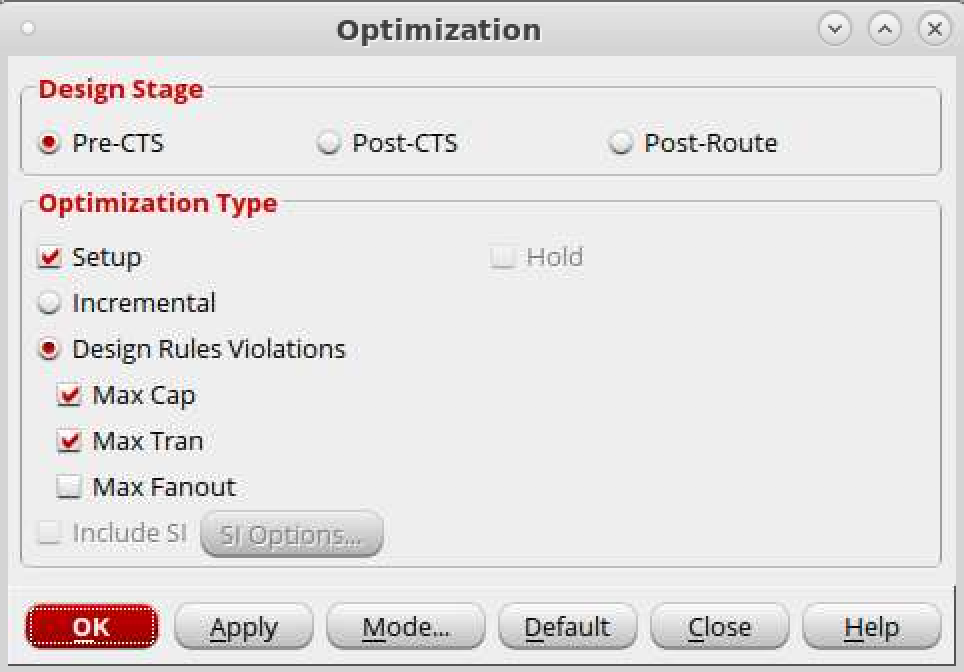
\includegraphics[scale=0.4]{figures/lab5_backend/optimize_prects}
			\caption{Optimizing the design.}
			\label{optimize_prects}
		\end{wrapfigure}
		\item Go to: \textit{ECO -> Optimize Design...}
		\item Select \textit{Pre-CTS} as in Fig. \ref{optimize_prects} and click \textit{Ok}.
		\item When it is done, observe how the slack changed on the terminal. Depending on if you had a large slack or a negative slack, the optimization results can be very different. If you had a large slack, the tool will not be able to optimize a lot since the design already meets the timing constraints easily. 
		\begin{codeline}
			optDesign -preCTS
		\end{codeline}
		
		\item Save your design as \textit{DBS/mips$\_$place.enc}, as explained in Section \ref{save}.
		
				\begin{codeline}
		saveDesign DBS/mips$\_$place.enc
		\end{codeline}
	} 

\end{enumerate}

	\begin{exercise}\
	\vspace{-6mm}
	\begin{enumerate}
		\item Report the critical path timing before and after optimization after the place step.
		\item During the optimization step, how do you think Innovus® optimized the design in order to improve the slack?
	\end{enumerate}
	\vspace{-5mm}
\end{exercise}
\clearpage

\subsection{Synthesizing the Clock Tree}
Since the paths propagating the \textit{clock} signal are not all balanced, some registers will receive the \textit{clock} signal after or before the others. If that happens, that means that the design would not be synchronous anymore. To correct this, the tool will insert some inverters in the design to add some delay so each register will receive the \textit{clock} signal at the same time. First, you can take a quick look at the initial clock tree as follow:


\begin{enumerate}
	\parbox[t]{\dimexpr\textwidth-\leftmargin}{%		
	\begin{wrapfigure}[20]{r}{0.45\textwidth}
		\vspace{0mm}
		\centering
		\vspace{-\baselineskip}
		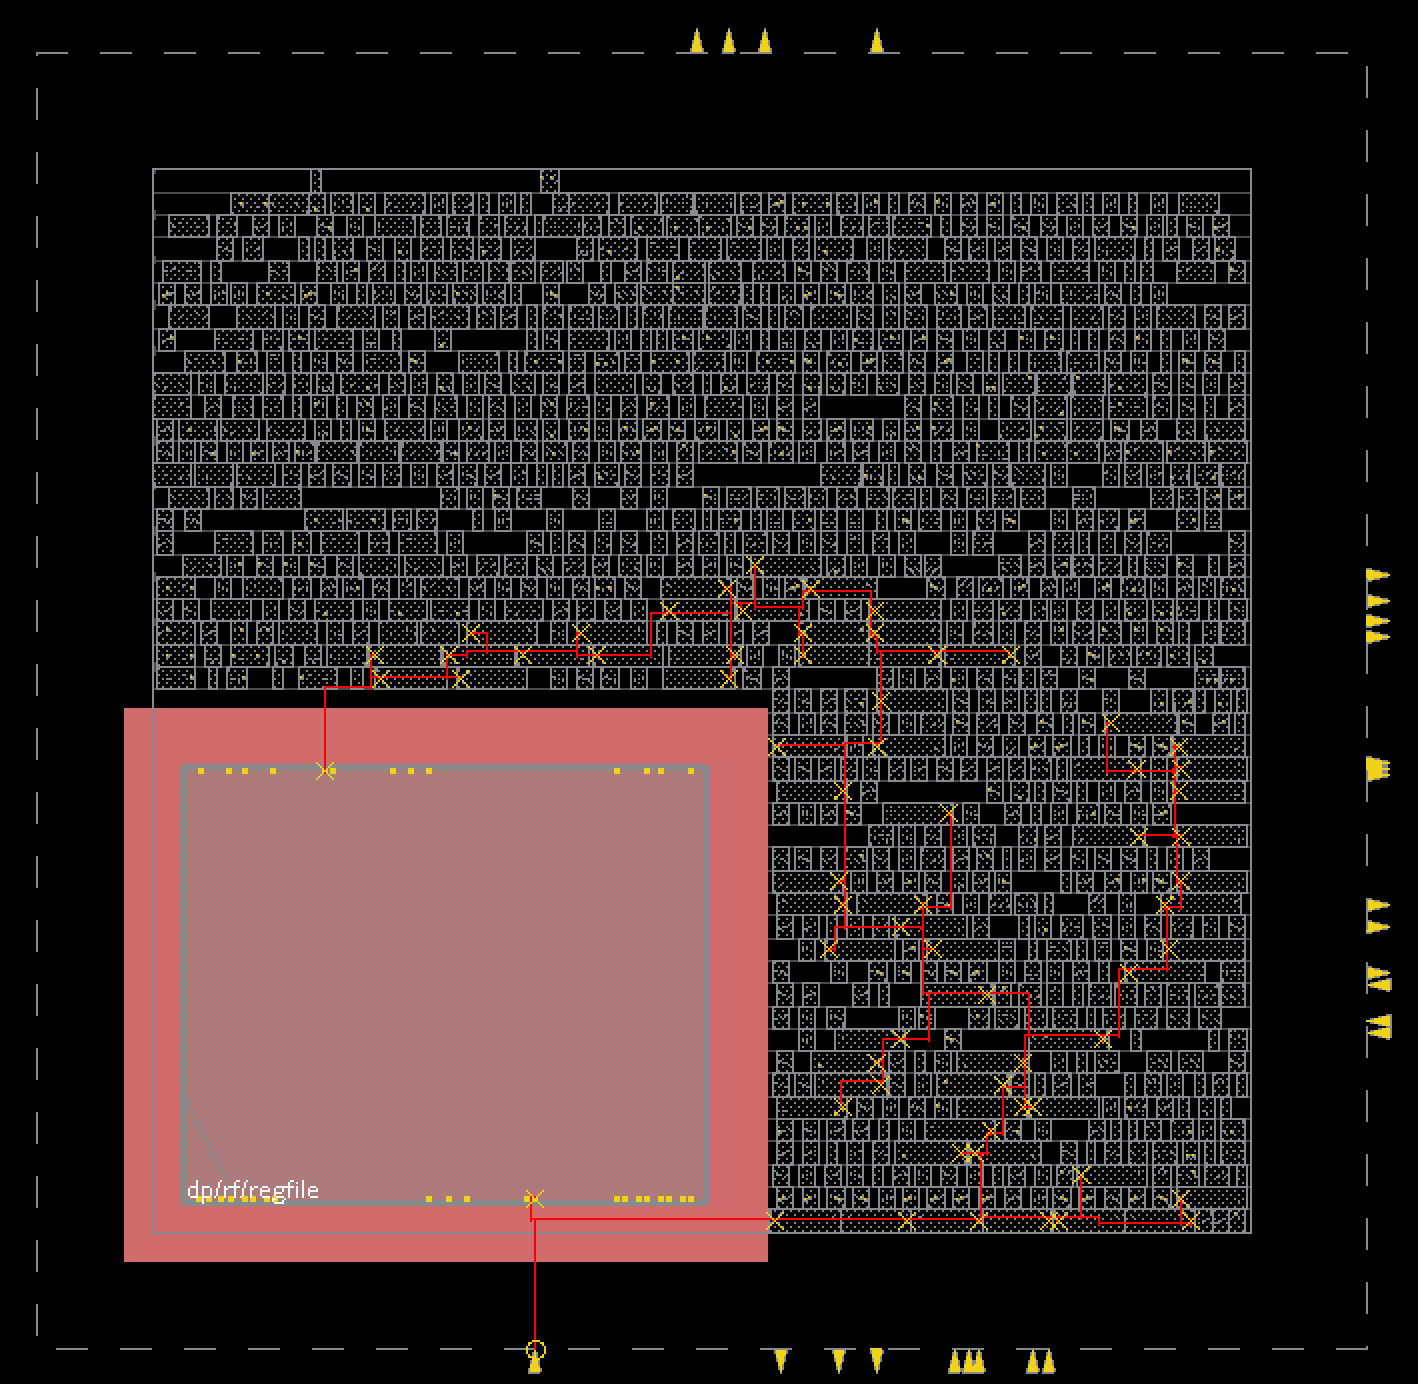
\includegraphics[scale=0.3]{figures/lab5_backend/clock_tree_view}
		\caption{Clock tree path.}
		\label{clock_tree_view}
	\end{wrapfigure}
\item Go to \textit{Tools -> Design Browser...}.
\item Under \textit{Nets}, select \textit{clk}.
\item On the visibility toggles (on the right part of the screen, as explained in Fig. \ref{fig_main_window}), deselect \textit{Net} and \textit{Cell} and select the \textit{Floorplan} view. That way, you can see the clock tree, as depicted in Fig. \ref{clock_tree_view}.
\item Before going to the next step, don't forget to select back the \textit{Net} and \textit{Cell} fields in the visibility toggles.
\item Before synthesizing the clock tree, several options can be performed such as specifying the list of usable inverters or buffers or specifying the width and spacing of the metals the clock tree should use. In this lab, we will use the default settings so there is nothing to specify. To do the \textit{Clock Tree Synthesis} (CTS), do:
		\begin{codeline}
ccopt$\_$design –cts
\end{codeline}} 

\begin{exercise}
Report the critical path timing before and after optimization after the CTS step, for both setup and hold mdoes (you will have to report the timing twice). Do not forget to select the appropriate \textit{Design Stage} for both the \textit{Timing Analysis} and \textit{Optimization} windows since the CTS step is now done. \textbf{When optimizing the design, select both setup and hold fields in the \textit{Optimization Type} field.}

\begin{codeline}
timeDesign -postCTS \\
timeDesign -postCTS -hold \\
optDesign -postCTS -setup -hold
\end{codeline}


\end{exercise}
\item Save your design as \textit{DBS/mips$\_$cts.enc}, as explained in Section \ref{save}. 

\begin{codeline}
	saveDesign DBS/mips$\_$cts.enc
\end{codeline}
\end{enumerate}



\clearpage

\subsection{Routing the Design}
This step will connect all your standard cell together as well as the I/O pins and will create the resulting wires. To route your design:


\begin{enumerate}
	\parbox[t]{\dimexpr\textwidth-\leftmargin}{%		
		\begin{wrapfigure}[20]{r}{0.45\textwidth}
			\vspace{0mm}
			\centering
			\vspace{-\baselineskip}
			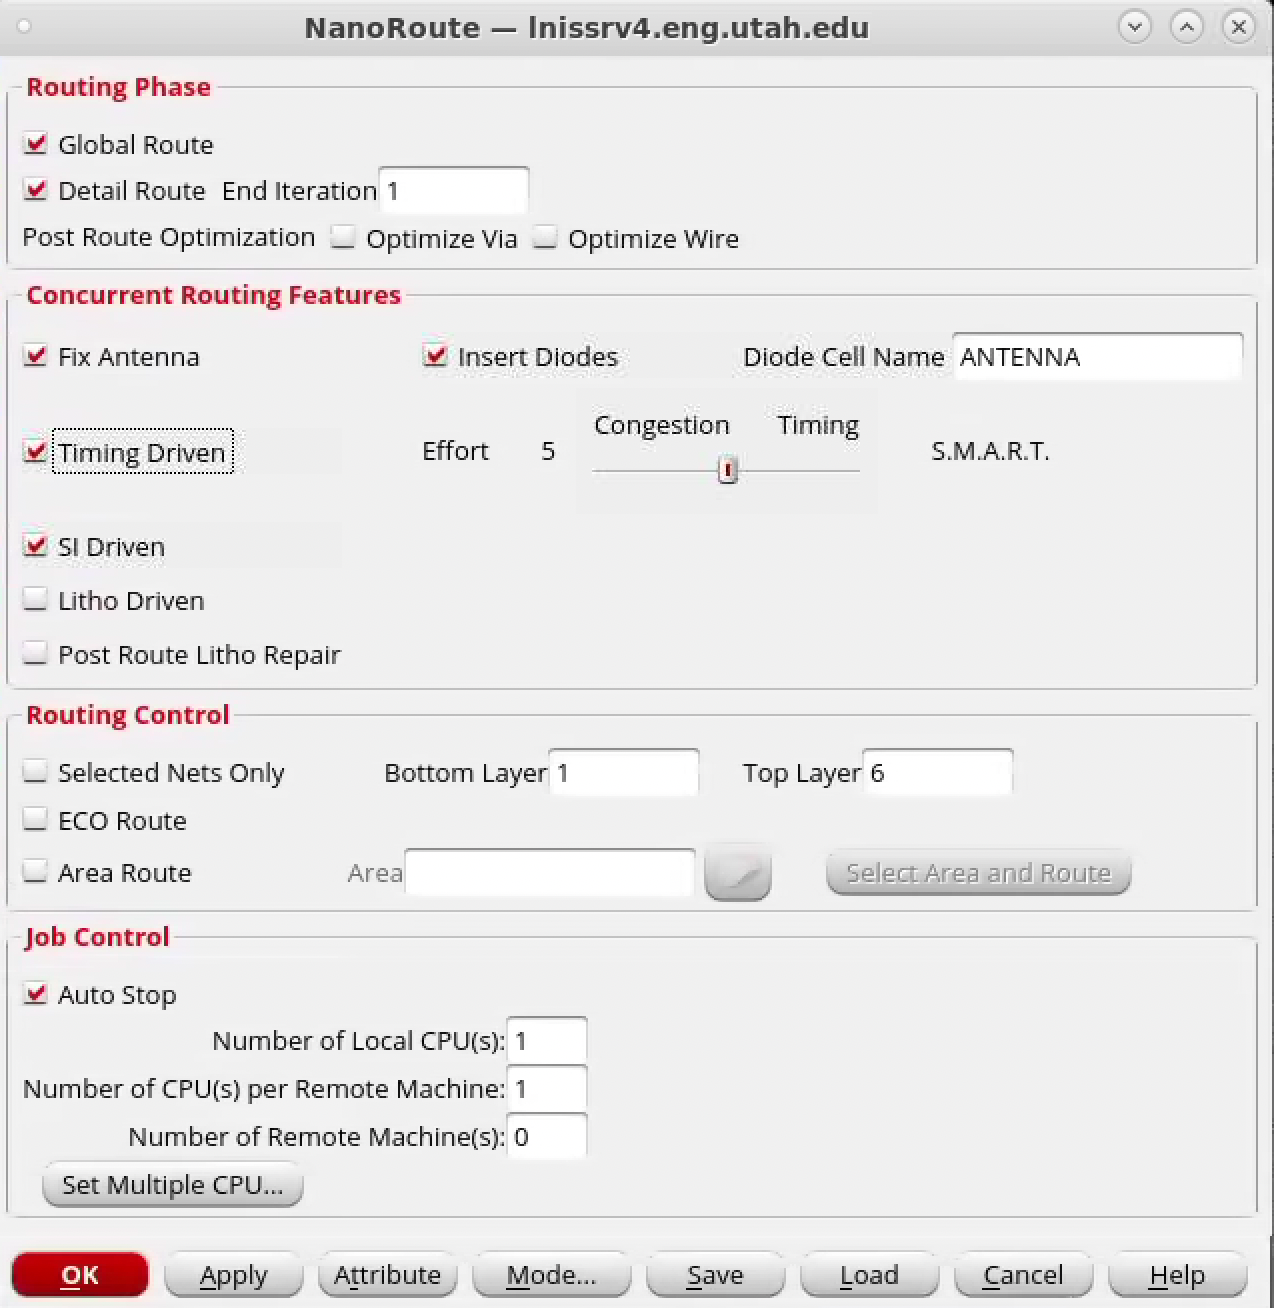
\includegraphics[scale=0.3]{figures/lab5_backend/route_options}
			\caption{Routing option window.}
			\label{route_options}
		\end{wrapfigure}
		\item Go to \textit{Route -> NanoRoute -> Route...}.
		\item Select the same options as in Fig. \ref{route_options}.
		\item Click on \textit{OK}. \\ \\
		Equivalent Innovus command:
		\begin{codeline}
		setNanoRouteMode $\textbackslash$\\‐routeWithTimingDriven true $\textbackslash$ ‐routeTdrEffort 5 $\textbackslash$\\ -routeWithSiDriven true $\textbackslash$\\ -drouteFixAntenna true $\textbackslash$ \\-routeInsertAntennaDiode true $\textbackslash$ \\-routeAntennaCellName ANTENNA \\
routeDesign ‐globalDetail ‐wireOpt $\textbackslash$\\‐viaOpt
		\end{codeline}
		\item You can now observe the final routed design on the design display area.
	} 
\item As before, report the timing (and select the \textit{Post-Route} option). If necessary, optimize your design as before.

\begin{codeline}
setAnalysisMode -analysisType onChipVariation \\
timeDesign -postRoute \\
timeDesign -postRoute -hold \\
optDesign -postRoute -setup -hold
\end{codeline}



\item Save your design as \textit{DBS/mips$\_$route.enc}, as explained in Section \ref{save}. 
\begin{codeline}
	saveDesign DBS/mips$\_$route.enc
\end{codeline}

\end{enumerate}


\clearpage
\subsection{Adding the Filler Cells}
Since you specified a core utilization of 80$\%$, there is still some empty space in your design. The ensure the continuity of the doping and well zones, some filler cell (which do not have any logic function) have to be adder.


\begin{enumerate}
	\parbox[t]{\dimexpr\textwidth-\leftmargin}{%		
		\begin{wrapfigure}[20]{r}{0.7\textwidth}
			\vspace{0mm}
			\centering
			\vspace{-\baselineskip}
			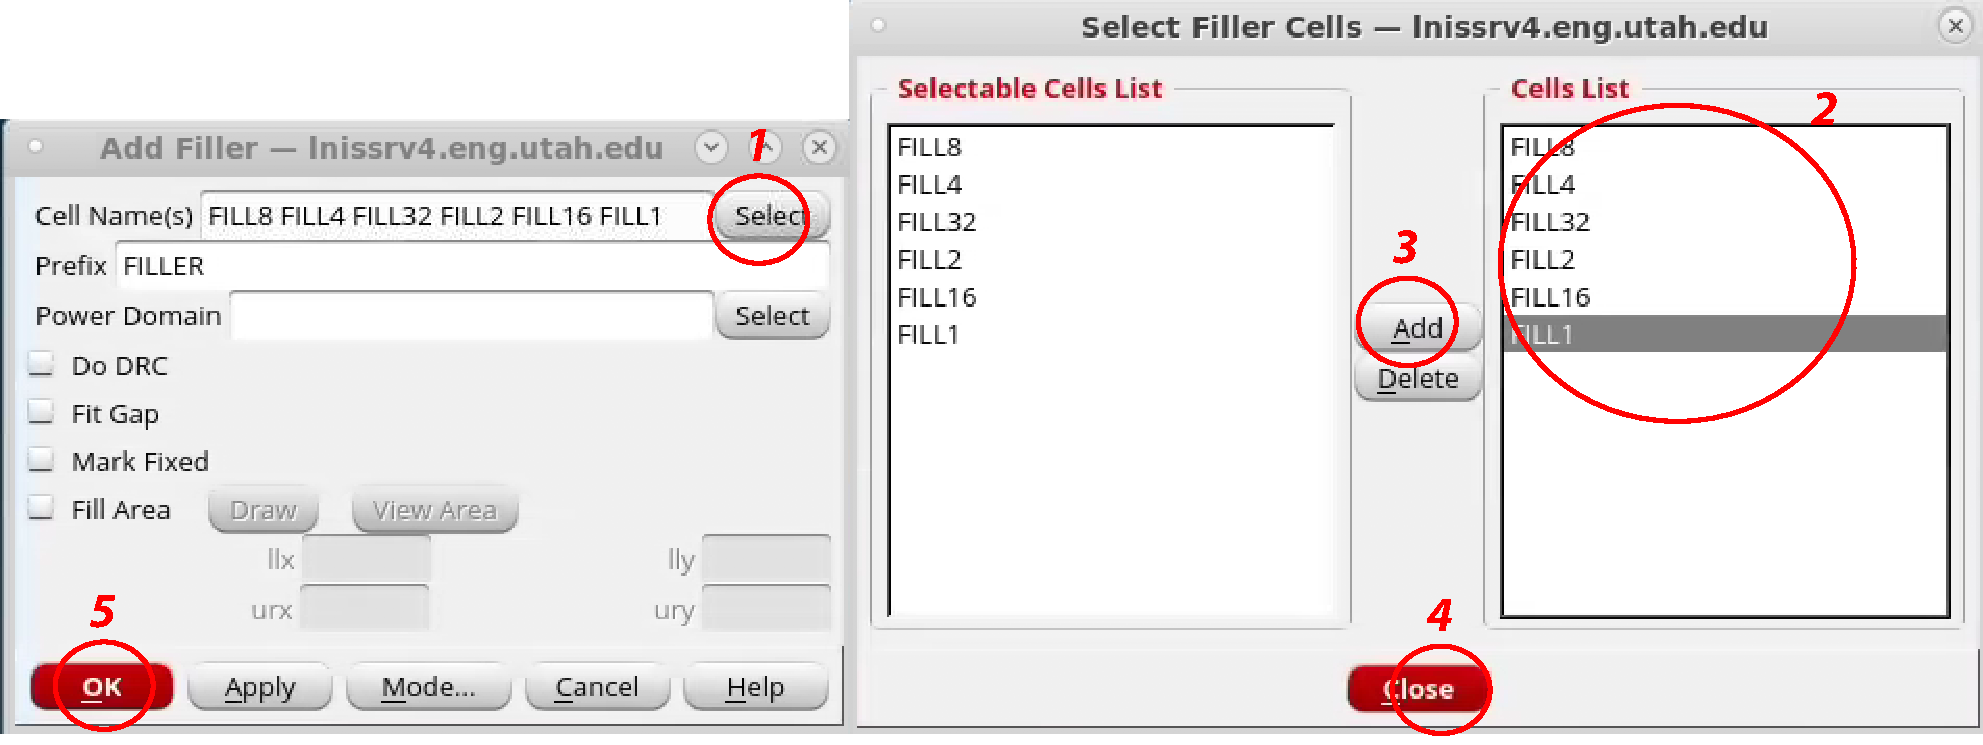
\includegraphics[scale=0.36]{figures/lab5_backend/addfiller}
			\caption{Adding the filler cells.}
			\label{fillercells}
		\end{wrapfigure}
		\item Go to \textit{Place -> Physical Cell -> Add Filler...}.
		\item Click on the \textit{Select} button and choose the appropriate filler cells in the list, as in Fig. \ref{fillercells}.
		\item Click on \textit{Close} and then \textit{OK}.
	} 

			\vspace{8mm}
			Equivalent Innovus command:
		\begin{codeline}
	addFiller -cell FILL32 FILL16 FILL8 FILL4 FILL2 FILL1 -prefix FILLER
\end{codeline}
		\item Observe the new layout. There should not be any empty space anymore. You can also look at the console which displays which filler cells have been added.
\item Save your design as \textit{DBS/mips$\_$fill.enc}, as explained in Section \ref{save}. 
\begin{codeline}
	saveDesign DBS/mips$\_$filler.enc
\end{codeline}
\end{enumerate}


\subsection{Verifying the Design}
\subsubsection{Verifying the Connectivity}

\begin{enumerate}
	\parbox[t]{\dimexpr\textwidth-\leftmargin}{%		
	\begin{wrapfigure}[20]{r}{0.33\textwidth}
		\vspace{-6mm}
		\centering
		\vspace{-\baselineskip}
		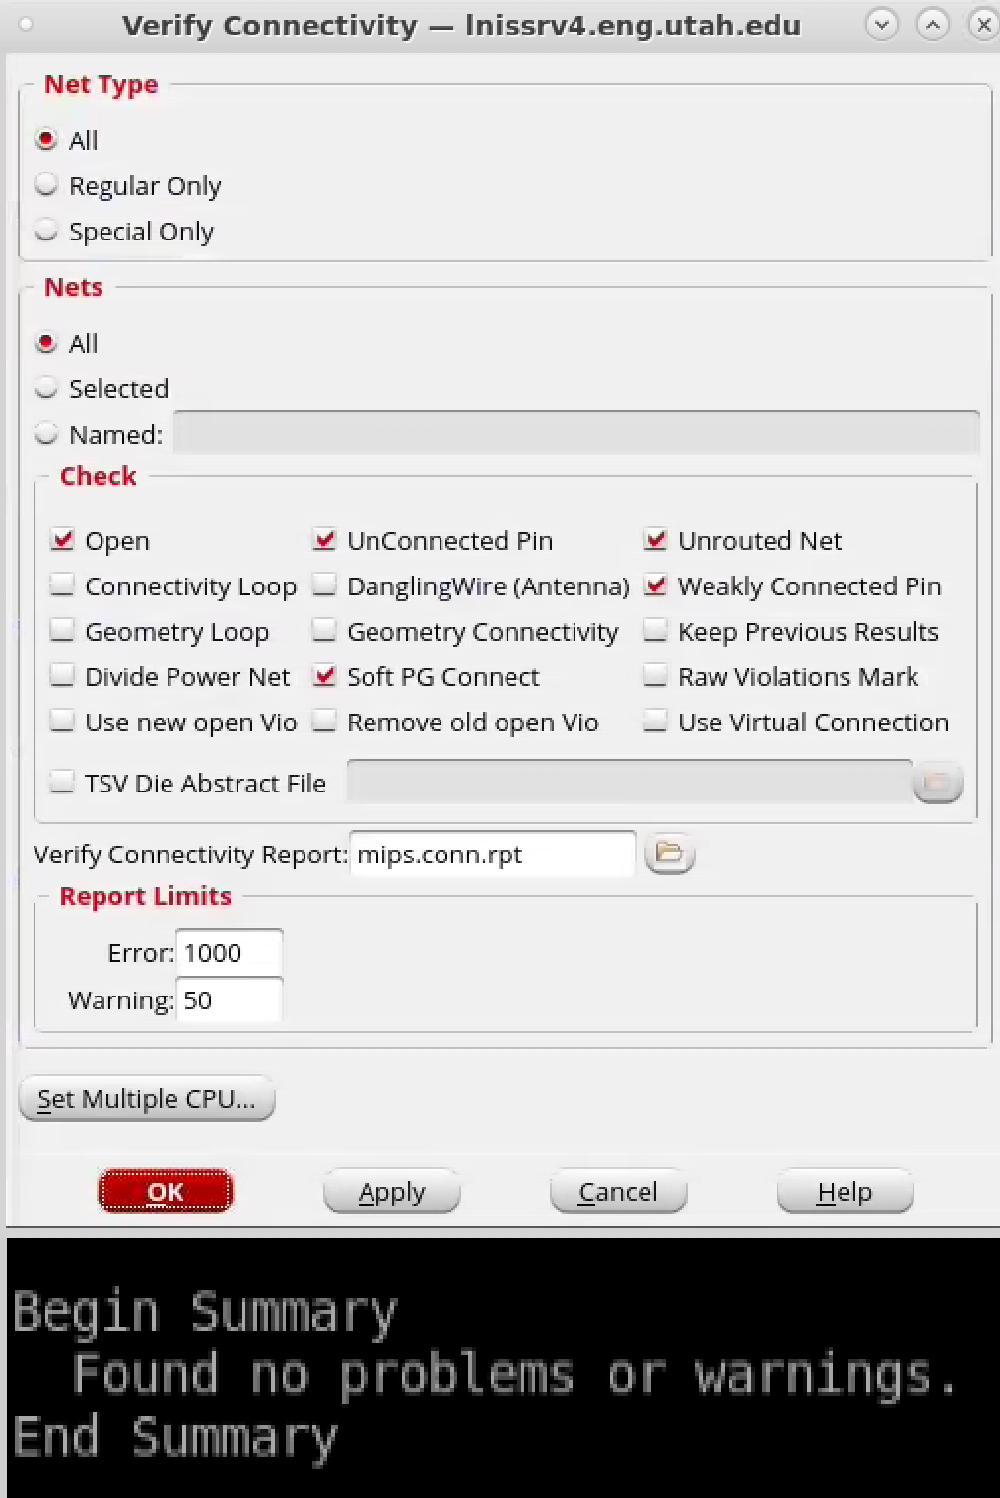
\includegraphics[scale=0.3]{figures/lab5_backend/verify_connect.pdf}
		\caption{Verifying the connectivity.}
		\label{verifyconnect}
	\end{wrapfigure}
This step will check your design for open or unconnected wires, unconnected pins, partial routing or unrouted nets.
	\item Go to \textit{Verify -> Verify Connectivity...}.
\item Select the same options, as shown in Fig. \ref{verifyconnect}.
	\item Specify the \textit{Verify Connectivity Report} as \textit{RPT/mips$\_$conn.rpt} in case you want to save the report.
	\item Click \textit{Ok}.
	\item Check the console terminal for possible errors. \\ \\
	Equivalent Innovus command:
	\begin{codeline}
		verifyConnectivity -noAntenna ‐type all $\backslash$ \\ ‐report RPT/mips$\_$conn.rpt
		‐error 1000 $\backslash$ \\ ‐warning 50
	\end{codeline}


} 

\end{enumerate}	

		\vspace{0mm}

\subsubsection{Verifying the Geometry}

\begin{enumerate}
	\parbox[t]{\dimexpr\textwidth-\leftmargin}{%		
	\begin{wrapfigure}[12]{r}{0.33\textwidth}
		\vspace{-6mm}
		\centering
		\vspace{-\baselineskip}
		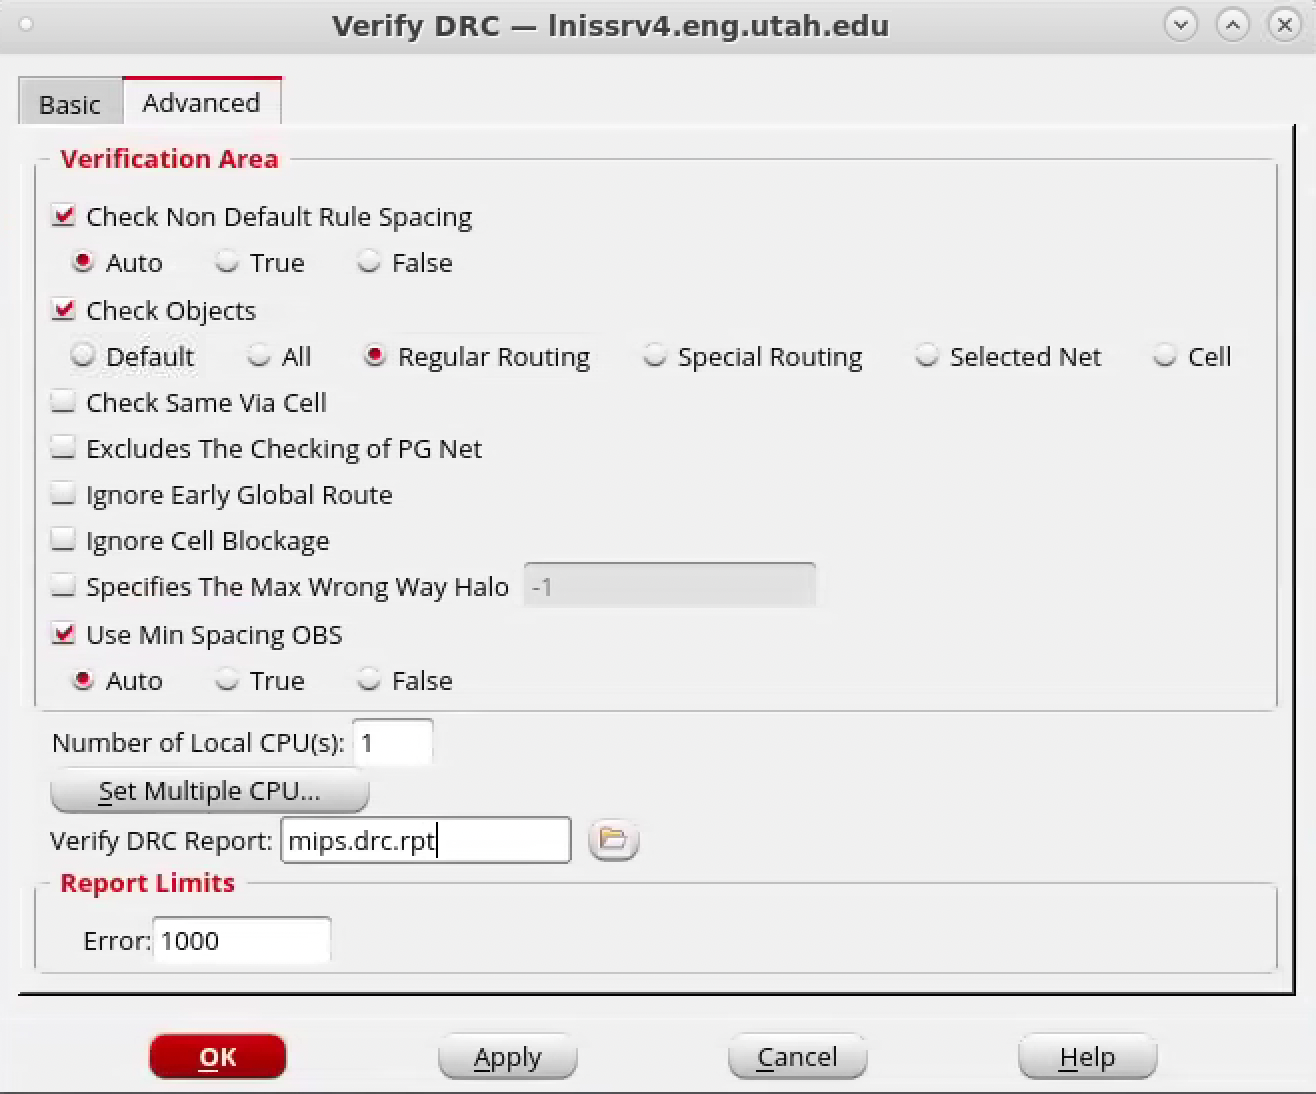
\includegraphics[scale=0.3]{figures/lab5_backend/verify_drc}
		\caption{Verifying the geometry.}
		\label{fillercells}
	\end{wrapfigure}
This step will check several DRC rules such as the metal minimum widths, shorts, minimum cut, \textit{etc.}
		\item Go to \textit{Verify -> Verify DRC...}.
		\item Specify the \textit{Verify DRC Report} field in the \textit{Advanced} tab as \textit{RPT/mips$\_$drc.rpt} in case you want to save the report.
		\item In the \textit{Advanced} tab, check the \textit{Regular Routing} option under \textit{Check Objects}.
		\item Click \textit{Ok}.
		\item Check the console terminal for possible errors. \\ \\
		Equivalent Innovus command:
		\begin{codeline}
		set$\_$verify$\_$drc$\_$mode -check$\_$only regula \\
verify$\_$drc ‐report RPT/mips$\_$geo.rpt

		\end{codeline}
		

} 
	\end{enumerate}


\begin{exercise}
	If you were to have a lot of DRC errors after your P$\&$R flow due to many metal wires being to close to each other, what could you do to address this issue?
\end{exercise}

\begin{checkpoint}\label{check2}
	Please call an assistant and show him that your final design looks correct after the verifying steps.
\end{checkpoint}

\subsection{Generating the Reports}
The previous steps should have generated several reports in the \textit{RPT} folder. It is possible to generate additional report.
\subsubsection{Netlist Statistics}

	\parbox[t]{\dimexpr\textwidth-\leftmargin}{%		
	\begin{wrapfigure}[20]{r}{0.4\textwidth}
		\vspace{-10mm}
		\centering
		\vspace{-\baselineskip}
	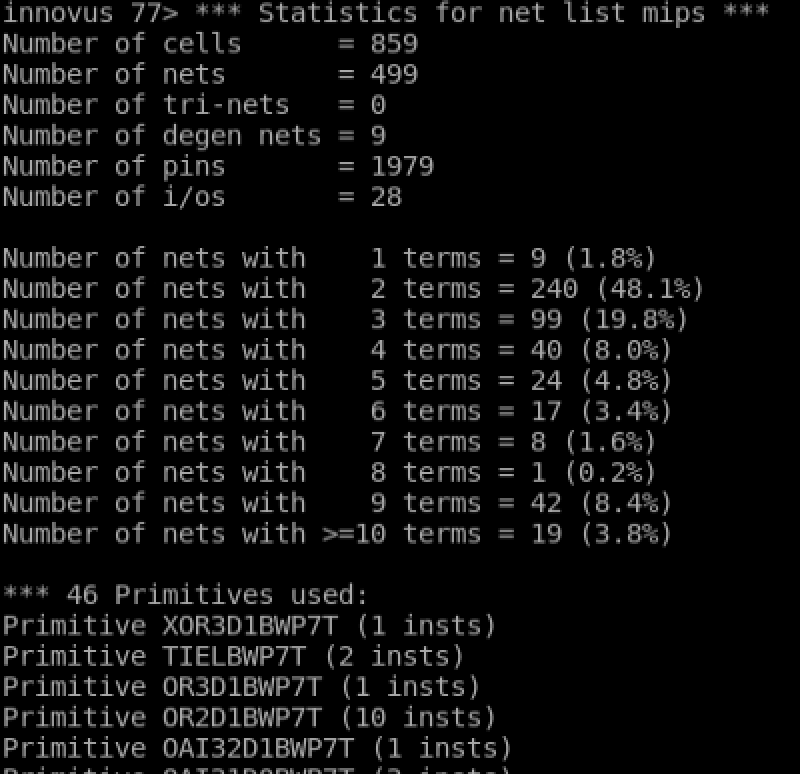
\includegraphics[scale=0.45]{figures/lab5_backend/netlist_stat}
\caption{Netlist statistic report.}
\label{netlist_stat}
	\end{wrapfigure}

Select \textit{File -> Report -> Netlist Statistics}. It will report several information about your design, as shown in Fig. \ref{netlist_stat}. Equivalent Innovus command:
\begin{codeline}
	reportNetStat
\end{codeline}
If you want to save the output somewhere, do:
\begin{codeline}
	reportNetStat >> RPT/name$\_$of$\_$your$\_$file
\end{codeline}
} 

		\vspace{6mm}
\subsubsection{Reporting the Critical Path}


To report the critical path timing, type in the terminal:
\begin{codeline}
	report$\_$timing
\end{codeline}


\begin{figure}[!h]
	\centering
	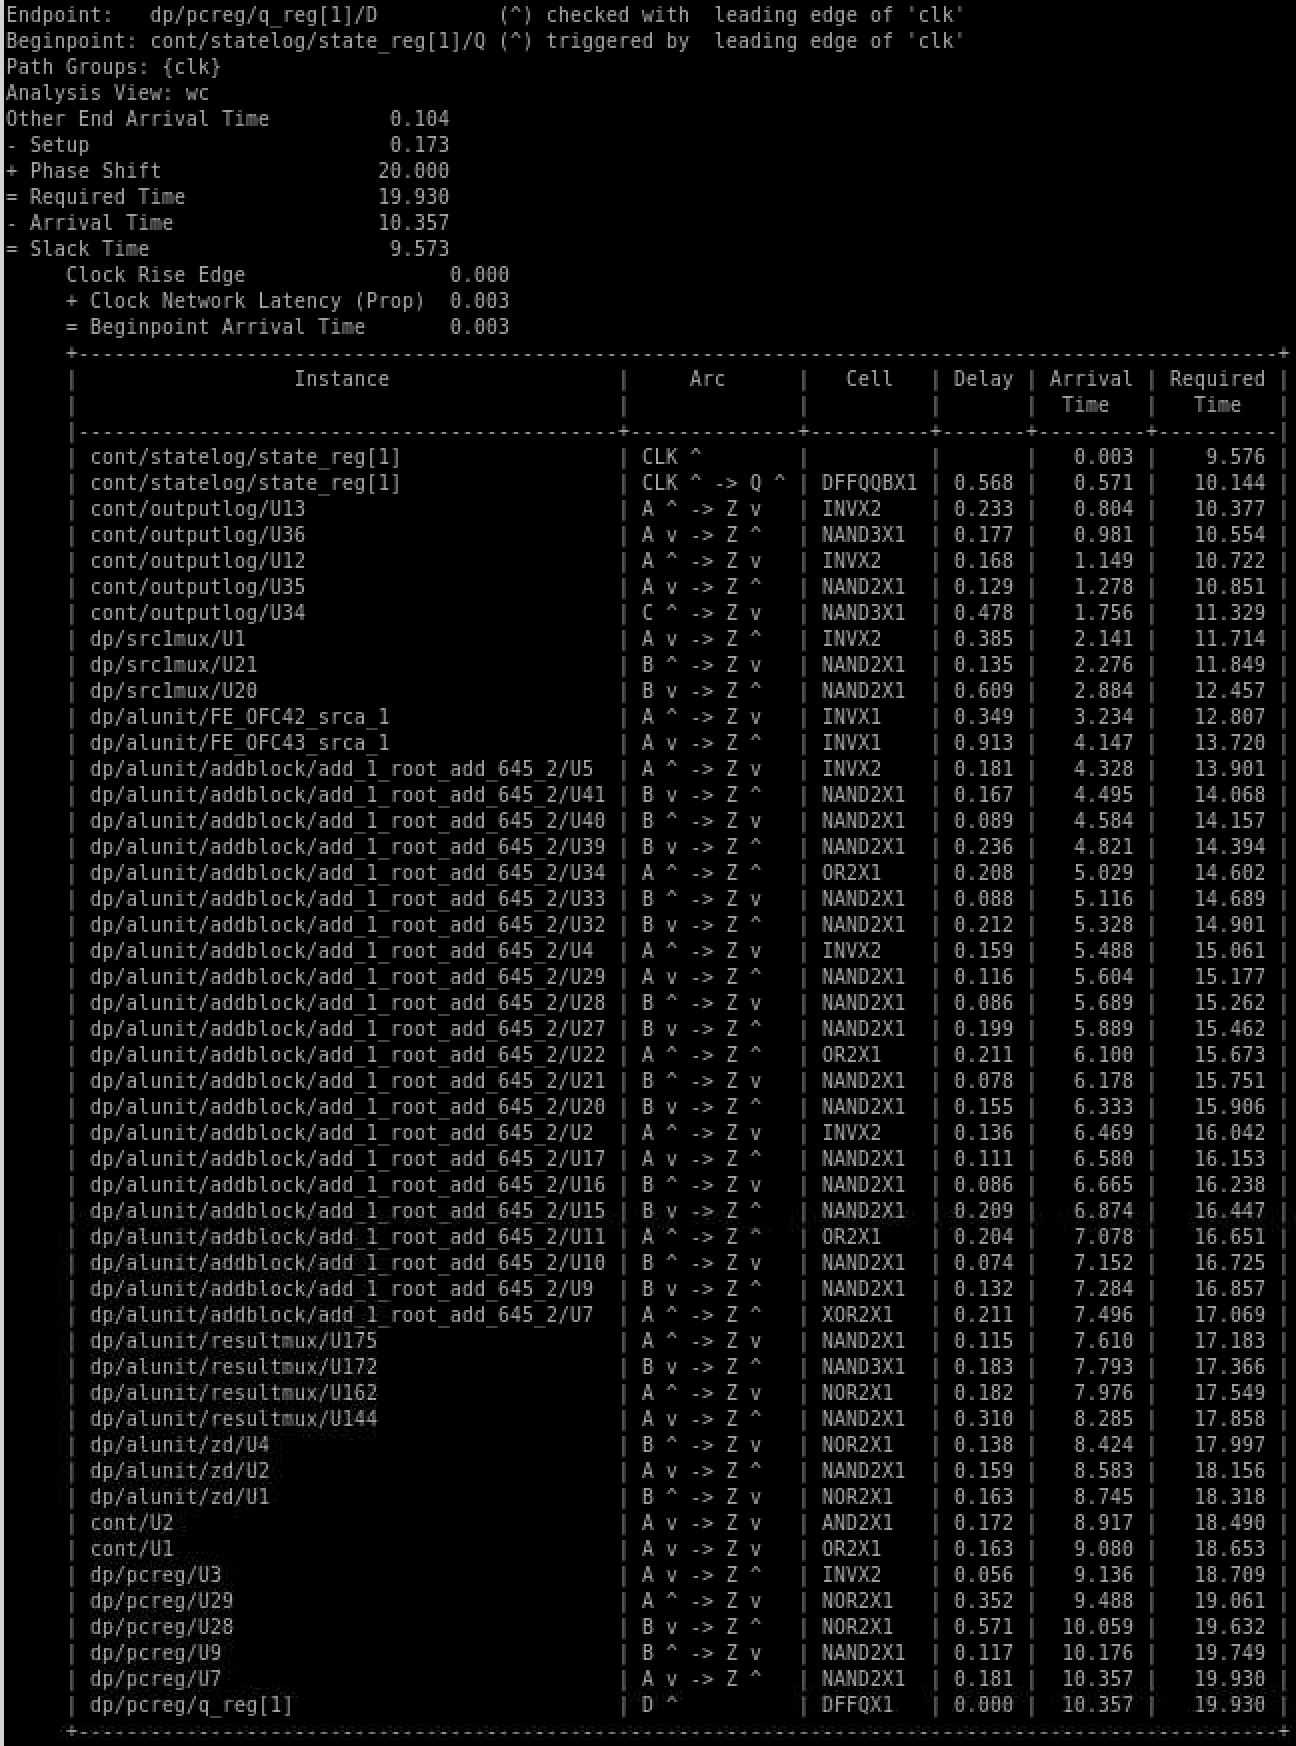
\includegraphics[scale=0.5]{figures/lab5_backend/report_timing}
	\caption{Critical path timing report.}
\end{figure}

\clearpage
\subsubsection{Reporting the Total Area}


To report the area of your design, type in the terminal:
\begin{codeline}
	report$\_$area
\end{codeline}
It will report the area of each module (\textit{mips} being the top module) and specify its hierarchy level.

\begin{figure}[!h]
	\centering
	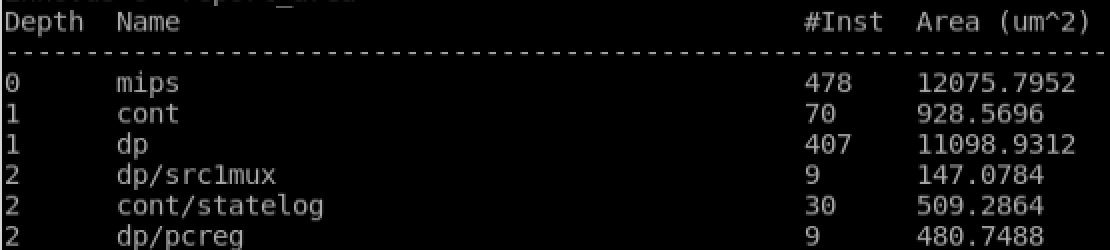
\includegraphics[scale=0.45]{figures/lab5_backend/report_area_inno}
		\caption{Area report.}
\end{figure}


\subsection{Exporting the Final Design}

\subsubsection{Generating the SDF timing file}
This step will generate the \textit{Standard Delay Format} (SDF) file which includes the gate and wire delays. It is then used for post-backend functional verification (with Modelsim\textsuperscript{\tiny\textregistered} for instance). To do so:

\begin{enumerate}
	\parbox[t]{\dimexpr\textwidth-\leftmargin}{%		
		\begin{wrapfigure}[12]{r}{0.33\textwidth}
			\vspace{-6mm}
			\centering
			\vspace{-\baselineskip}
	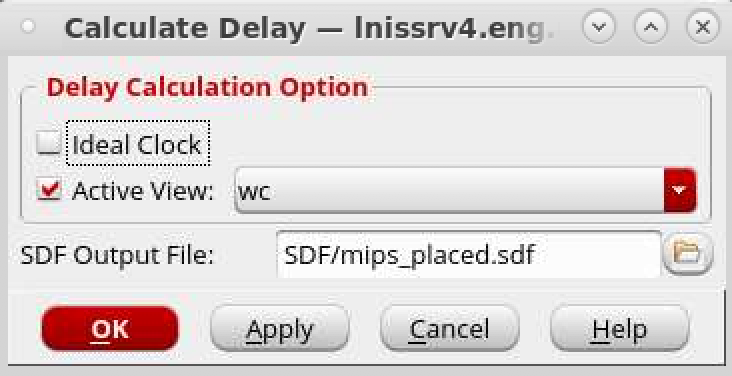
\includegraphics[scale=0.45]{figures/lab5_backend/write_sdf}
\caption{Writing the SDF file.}
			\label{write_sdf}
		\end{wrapfigure}
		\item Note: The SDF can only be exported if a timing analysis has been previously done (through \textit{TimeDesign} or \textit{report$\_$timing} for instance.
		\item Go to \textit{Timing  -> Write SDF...}
		\item Select the \textit{wc} active view (worst case, so for setup analysis).
		\item Specify the output file as SDF/mips$\_$placed.sdf
		\item Click \textit{Ok}.
	} 
	\vspace{6mm}
\end{enumerate}



Equivalent Innovus command:
\begin{codeline}
write$\_$sdf -view wc SDF/mips$\_$placed.sdf
\end{codeline}

\subsubsection{Generating the Verilog Gate-level Netlist}
As you did after the synthesis step, you can generate a verilog gate-level netlist after the P$\&$R flow. This netlist might differ from the initial netlist since some gates could have been resized or added (during the CTS for instance). To generate the file:

\begin{enumerate}
	\parbox[t]{\dimexpr\textwidth-\leftmargin}{%		
		\begin{wrapfigure}[12]{r}{0.33\textwidth}
			\vspace{-6mm}
			\centering
			\vspace{-\baselineskip}
			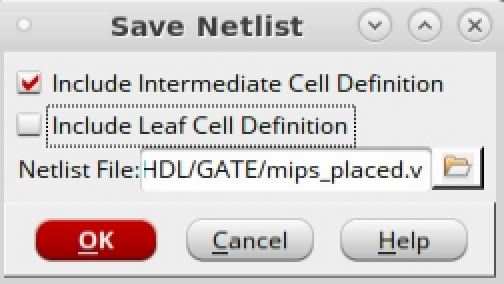
\includegraphics[scale=0.55]{figures/lab5_backend/save_netlist_placed}
			\caption{Generating the final verilog netlist.}
			\label{save_netlist_placed}
		\end{wrapfigure}
\item Go to \textit{File -> Save -> Netlist...}
\item Deselect the \textit{Include Leaf Cell Definition} field.
\item Specify the netlist file as HDL/GATE/mips$\_$placed.v
\item Click \textit{Ok}.
	} 
			\vspace{6mm}
\end{enumerate}
Equivalent Innovus command:
\begin{codeline}
saveNetList ‐excludeLeafCell HDL/GATE/mips.placed.v
\end{codeline}


\subsubsection{Generating the GDSII File}
The design can be exported as a GDSII file which is a binary file format representing the planar geometric shapes, text labels and other information about your design. It is generally used to be imported into Virtuoso\textsuperscript{\tiny\textregistered} or to be sent to the foundry for fabrication.

\begin{enumerate}
	\parbox[t]{\dimexpr\textwidth-\leftmargin}{%		
		\begin{wrapfigure}[16]{r}{0.4\textwidth}
			\vspace{-6mm}
			\centering
			\vspace{-\baselineskip}
			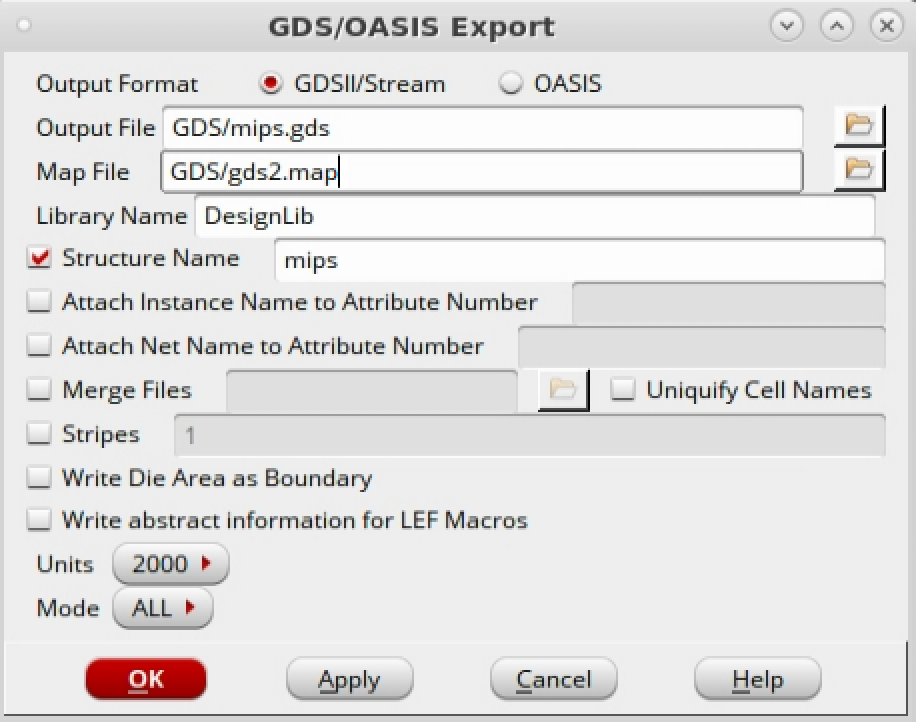
\includegraphics[scale=0.45]{figures/lab5_backend/export_gds}
			\caption{Generating the GDSII file.}
			\label{export_gds}
		\end{wrapfigure}
		\item Go to \textit{File -> Save -> GDS/OASIS...}
		\item As in Fig. \ref{export_gds}, fill out the appropriate fields.
		\item Click \textit{Ok}.
		\item Check in the terminal to verify that the \textit{Streamout} phase has been done without any issue. \\
		Equivalent Innovus command:
		\begin{codeline}
			streamOut GDS/mips.gds -mapFile GDS/gds2.map -libName DesignLib -structureName mips -units 2000 -mode ALL
		\end{codeline}
	} 
\end{enumerate}


\subsection{Importing the Final Design into Virtuoso\textsuperscript{\tiny\textregistered}}
To import the design after the P$\&$R steps into Virtuoso\textsuperscript{\tiny\textregistered}:

\begin{enumerate}
	\item From the virtuoso CIW window, \textit{File -> Import -> Stream...}.
	\item In the \textit{XStream In} window, specify the path of your GDSII file (which should be in the \textit{GDS} folder of your \textit{innovus} directory) as the \textit{Stream File}.
	\item Specify a library name. If this library does not exist, it will be created.
	\item Specify the \textit{Top Cell} name which should match the one you used when exporting the GDSII file from Innovus\textsuperscript{\tiny\textregistered}.
	\item In the \textbf{Technology} tab, select \textit{tsmc18} so your new library will be attached to the TSMC 180nm technology library.
	\item Click on \textit{More Options}. Next to the \textit{Ref Lib File Name}, click on \img{figures/lab5_backend/new_icon}. Select the \textit{SC$\_$LIB} library and click on the right arrow. Do the same for the \textit{PADS$\_$LIB} and \textit{rf2hsm1wm1} libraries. This will ensure that this standard cell library is linked to your design during the importation phase. Since your top design is using many of those cells, they would be considered as black boxes otherwise. Click on \textit{Save As and Exit}, set the file name to \textit{reflib.list} and click on \textit{Save}.
	\item Click on \textit{Ok} then on \textit{Translate} in the XStream In window.
	\item The translation should start and you should not get any error.
\end{enumerate}

\begin{figure}[!h]
	\centering
	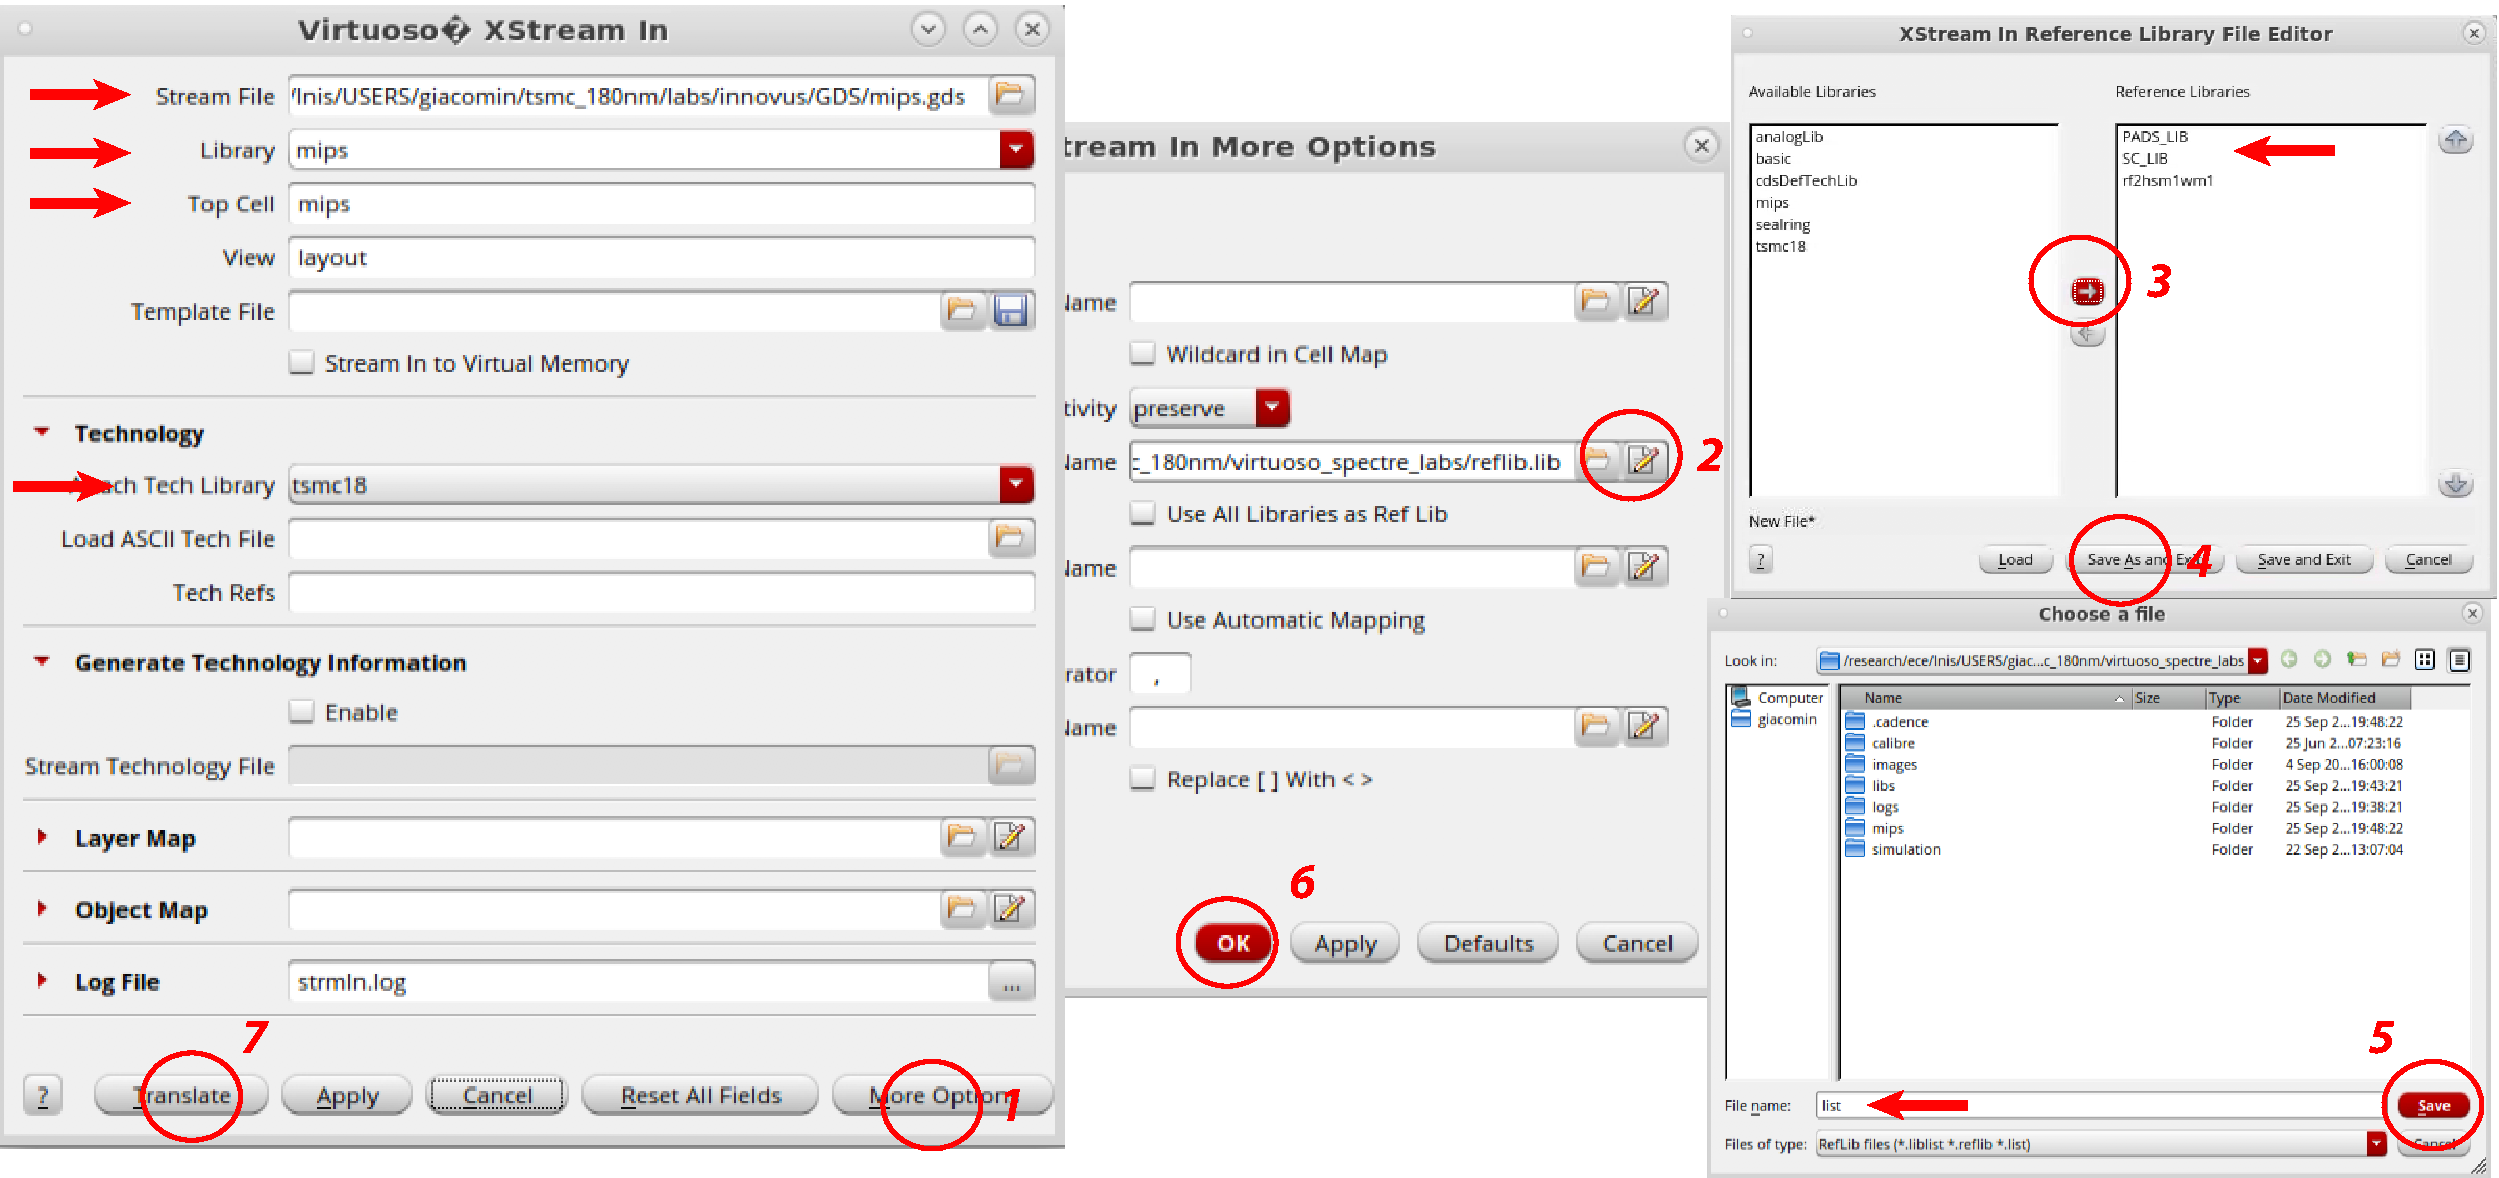
\includegraphics[scale=0.45]{figures/lab5_backend/import_gds.pdf}
	\caption{Importing a GDSII file into Virtuoso\textsuperscript{\tiny\textregistered.}}
	\label{import_gds}
\end{figure}

Now, go to the \textit{Library Manager} and open the \textit{mips} layout view in your newly imported library. You should obtain something similar as Fig. \ref{mips_virtuoso}. If you only see metal wires, do \textbf{Shift+F} to also display the cells and the IP. If you zoom in, you can see all the standard cells from the standard cell library. As you can see, only the metal layers are shown for the IP block and nothing about the transistor or doping layers. This is because the companies selling IPs generally only provide \textit{abstract} views for the P$\&$R flow (which just needs the metal information from the standard cells) for confidentiality reasons.
\begin{figure}[!h]
	\centering
	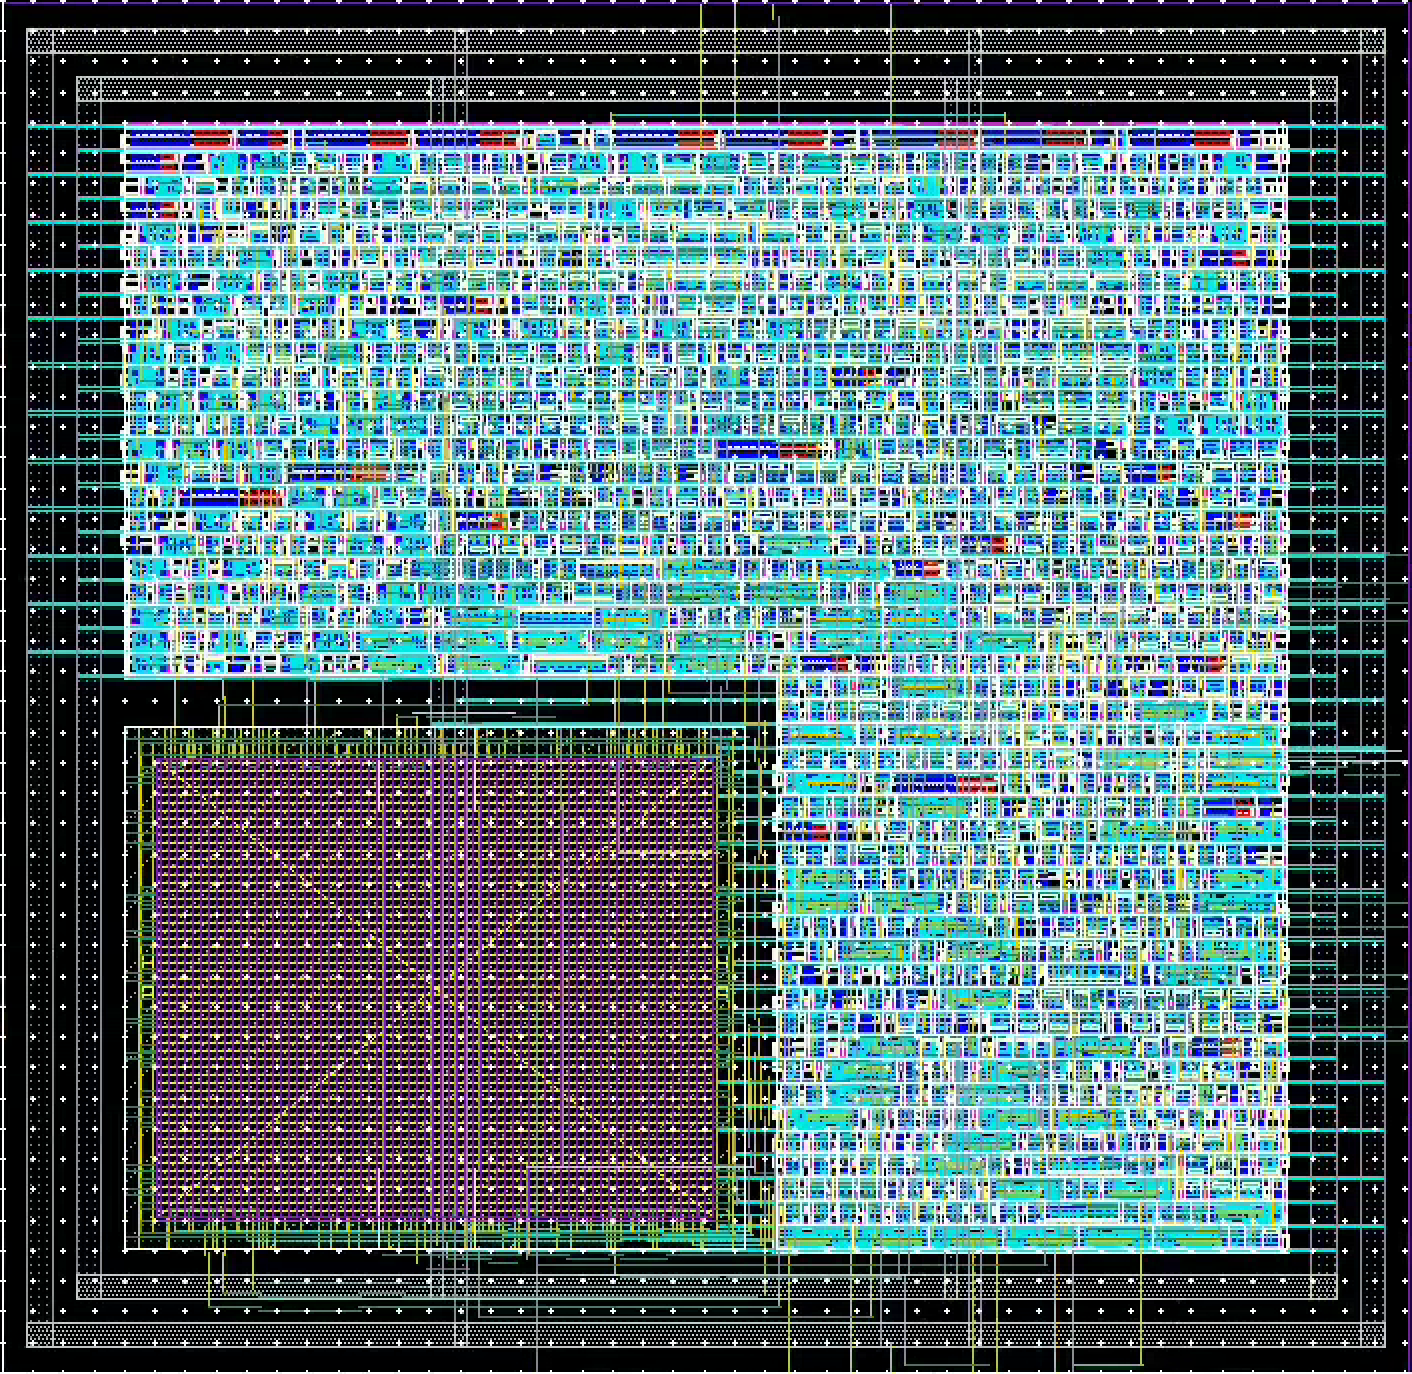
\includegraphics[scale=0.4]{figures/lab5_backend/mips_virtuoso}
	\caption{MIPS layout view from Virtuoso\textsuperscript{\tiny\textregistered.}}
	\label{mips_virtuoso}
\end{figure}
			\vspace{-6mm}

\subsubsection{Using a TCL script}
As in the previous lab, instead of using the GUI, you could use a \textit{.tcl} script to automatize your flow and optimize your design with tighter time constraints. The \textit{place$\_$route.tcl} script in your \textit{innovus/SCRIPTS} directory contains all the commands of this lab. Open it and take a look at how it is organized. You can see that it contains several procedures, each of which will perform one step (importing the design, saving the design, place, route, CTS, \textit{etc.}). Try to understand what each procedure is for, you should recognize most of the commands used in this lab. Also, pay attention where each report is created at the end of each step (more particularly for the \textit{generate$\_$reports} step). In each procedure, many variables are defined and then passed as parameters for the common Innovus commands\textsuperscript{\tiny\textregistered.}. The main procedure is called: \textbf{do$\_$steps} and has two arguments:  \textit{first$\_$step} \textit{last$\_$step}. Look at the very end of the \textit{place$\_$route.tcl} to see how it is defined: by passing only one argument number (2 for instance), a single step is performed (\textit{floorplan$\_$design} in this case). By passing two arguments (1 6 for instance), several steps are performed in order (\textit{init$\_$design} to \textit{route$\_$power$\_$nets} for instance). In order to use this script, launch Innovus\textsuperscript{\tiny\textregistered.} and do:

\begin{codeline}
source SCRIPTS/place$\_$route.tcl \\
set$\_$design mips
\end{codeline}

One way to do the whole flow would be to do:

\begin{codeline}
do$\_$steps 1 12
\end{codeline}

For the first time, it is advised to run the steps 1 by 1, to ease the debugging:
\begin{codeline}
	do$\_$steps 1 \\
		do$\_$steps 2 \\
			do$\_$steps 3 \\
			...
\end{codeline}

If something is not working, check the terminal as it will indicate what went wrong and try to understand what is the issue and how to address it. Sometimes, a file name has not been specified correctly, or you could have forgotten to specify the \textit{design$\_$name} for instance. Some common errors could come from your \textit{mips$\_$final.globals} file which defines the path of many configuration file. The latter file depends on the \textit{mips.view}, located in the \textit{/research/ece/lnis-teaching/5710$\_$6710$\_$F20/Lab$\_$files/innovus/CONF/} directory. This \textit{view} file depends on your constraint file generated after synthesis, so if you specified a wrong name, your P$\&R$ flow could go wrong.

	\begin{exercise}\
	\vspace{-6mm}
	\begin{enumerate}
		\item Try to optimize your design by specifying a tighter clock constraint (to do so, you will need re-synthesized it with the same clock constraint using the script of the previous lab). Do not forget to choose the appropriate \textit{.sdc} and verilog gate-level netlist files when importing your design since they depends on the clock constraint.
\item Report the minimum clock period you achieved and its associated critical path, total number of cells as well as its total area (provide some screenshots of the appropriate reports).
	\end{enumerate}
	\vspace{-5mm}
\end{exercise}


\section{Assignment and Checkpoint Summary}
Write a report and answer the assignments asked during the lab, which are summarized below. Do not forget to validate the checkpoints, summarized below as well, by an assistant before the end of the lab.

\begin{exercisesum}\	
	\vspace{-2mm}
	\begin{enumerate}
		\item Which metal layers should be used for power routing and for the \textit{Clock Tree Synthesis} (CTS) and why (it is not necessarily the default one used in this lab)?
		\item Report the critical path timing before and after optimization after the place step.
		\item During the optimization step, how do you think Innovus\textsuperscript{\tiny\textregistered} optimized the design in order to improve the slack?
		\item Report the critical path timing before and after optimization after the CTS step. Do not forget to select the appropriate \textit{Design Stage} for both the \textit{Timing Analysis} and \textit{Optimization} windows since the CTS step is now done. \textbf{When optimizing the design, select both setup and hold fields in the \textit{Optimization Type} field.}
		\item If you were to have a lots of DRC errors after your P$\&$R flow due to many metal wires being to close to each other, what could you do to address this issue?
		\item Try to optimize your design by specifying a tighter clock constraint (to do so, you will need re-synthesized it with the same clock constraint using the script of the previous lab). Do not forget to choose the appropriate \textit{.sdc} and verilog gate-level netlist files when importing your design since they depends on the clock constraint.
		\item Report the minimum clock period you achieved and its associated critical path, total number of cells as well as its total area (provide some screenshots of the appropriate reports). 
	\end{enumerate}
	\vspace{-5mm}
\end{exercisesum}	


\begin{checkpointsum}\
	\vspace{-2mm}
	\begin{enumerate}
		\item Please call an assistant and show him that your floorplan looks correct.
		\item Please call an assistant and show him that your final design looks correct after the verifying steps.
	\end{enumerate}
	\vspace{-5mm}
\end{checkpointsum}